
\documentclass[12pt, a4paper]{article}

\usepackage{graphicx}
\usepackage{xcolor}
\usepackage{float}
\usepackage{svg}
\usepackage[colorlinks=true, linkcolor=black, urlcolor=blue, citecolor=green]{hyperref}
\usepackage{enumitem}
\usepackage[italian]{babel}
\usepackage{lastpage}  % Pacchetto per ottenere il numero totale delle pagine
\usepackage{fancyhdr}  % Pacchetto per personalizzare l'intestazione e il piè di pagina
\usepackage[margin=1in]{geometry}
\usepackage{array}
\newcolumntype{C}[1]{>{\centering\arraybackslash}p{#1}}
\newcolumntype{L}[1]{>{\raggedright\arraybackslash}p{#1}}
\graphicspath{ {images/} {../shared/images/} }
\definecolor{unipd}{HTML}{B5121B}

\addto\captionsitalian{\renewcommand{\contentsname}{Indice}}

\setcounter{secnumdepth}{5}
\setcounter{tocdepth}{5}
\makeatletter
\newcommand\subsubsubsection{\@startsection{paragraph}{4}{\z@}{-2.5ex\@plus -1ex \@minus -.25ex}{1.25ex \@plus .25ex}{\normalfont\normalsize\bfseries}}
\newcommand\subsubsubsubsection{\@startsection{subparagraph}{5}{\z@}{-2.5ex\@plus -1ex \@minus -.25ex}{1.25ex \@plus .25ex}{\normalfont\normalsize\bfseries}}
\makeatother

\pagestyle{fancy}% Imposta lo stile di pagina su "fancy"
\fancyhf{}% Cancella intestazioni e piè di pagina
\fancyfoot[C]{\thepage{} di \pageref{LastPage}} % Imposta il piè di pagina centrale come "numero pagina di totale pagine"
\renewcommand{\headrulewidth}{0pt} % Imposta la larghezza della linea di intestazione a 0 punti

\newcommand{\data}{}
\newcommand{\titolo}{Manuale Utente}
\newcommand{\responsabile}{Responsabile}
\newcommand{\verificatore}{Derek Gusatto}
\newcommand{\redattore}{Matteo Gerardin}
\newcommand{\uso}{Esterno}
\newcommand{\destinatari }{
    & Vimar S.p.A.  \\
    & Tullio Vardanega  \\
    & Riccardo Cardin  }
\newcommand{\abstractcontent}{abstract ...}

\begin{document}

\begin{minipage}[]{0.3\textwidth}
\includesvg[width=\linewidth]{pebkac.svg} 
\end{minipage}
\hspace{0.1\textwidth}
\begin{minipage}[]{0.6\textwidth}
  {\Large \textbf{PEBKAC}} \\
  Email: \href{mailto:pebkacswe@gmail.com}{pebkacswe@gmail.com} \\
  Gruppo: 11
\end{minipage}

\bigskip

\begin{minipage}[]{0.3\textwidth}
\includesvg[width=\linewidth]{logo_unipd.svg} 
\end{minipage}
\hspace{0.1\textwidth}
\begin{minipage}[]{0.6\textwidth}
  \textcolor{unipd}{
    \textbf{Università degli Studi di Padova} \\
    Corso di Laurea: Informatica \\
    Corso: Ingegneria del Software \\
    Anno Accademico: 2024/2025
  }
\end{minipage}


\bigskip
\bigskip
\bigskip
\begin{center}
  \Huge\textbf{Verbale Interno}

  \Large\textbf{\data}
\end{center}

\bigskip


\begin{center}
\textbf{Informazioni sul documento}: \\
\vspace{0.5cm}

\begin{tabular}{r|l}
    \textbf{Responsabile} & Tommaso Zocche \\ 
    \textbf{Verificatore} & Alessandro Benin \\ 
    \textbf{Redattore} & Tommaso Zocche \\ 
    \textbf{Uso} & Interno \\ 
    \textbf{Destinatari} & Tullio Vardanega \\ & Riccardo Cardin \\ 
\end{tabular}

\vfill

\textbf{Abstract}: \\
\vspace{0.5cm}
L'obiettivo dell'incontro è stato definire l'ordine di preferenza dei capitolati a seguito degli incontri avuti con le aziende interessate e iniziare a redigere il prospetto orario del gruppo.
\end{center}


\bigskip
\newpage

\section*{Registro delle modifiche}
\begin{table}[H]
    \begin{tabular}{|c|c|c|c|p{5cm}|}
        \hline
         \textbf{Versione} &  \textbf{Data} &  \textbf{Autore} &  \textbf{Ruolo} & \textbf{Descrizione} \\
          \hline
          &  &  & Responsabile & Approvazione e rilascio\\
          \hline
          0.1.0 & 17/11/2024 & Alessandro Benin & Verificatore  & Verificato \\
          \hline
          0.0.1 & 13/11/2024 & Derek Gusatto & Amministratore  & Stesura iniziale \\
          \hline
    \end{tabular}
\end{table}
\newpage
\tableofcontents
\newpage
% VERBALE
% \section{Informazioni generali}
\begin{itemize}
  \item \textbf{Tipo riunione}: esterna
  \item \textbf{Luogo}: telematica, Teams
  \item \textbf{Data}: 25 novembre 2024
  \item \textbf{Ora inizio}: 16.00
  \item \textbf{Ora fine}: 17.00
  
  \item \textbf{Presenti}:
  \begin{itemize}
    \item Alessandro Benin
    \item Ion Bourosu
    \item Matteo Gerardin
    \item Derek Gusatto
    \item Davide Martinelli
    \item Matteo Piron
    \item Tommaso Zocche
    \item[$\star$] Mariano Sciacco (Vimar S.p.A.)
    \item[$\star$] Francesca Stival (Vimar S.p.A.)
  \end{itemize}

  \item \textbf{Assenti}:
 
\end{itemize}
% \newpage
% \section{Riassunto della riunione}
Nella presente riunione ci siamo allineati sugli ultimi task mancanti per la candidatura alla prima revisione RTB, che il gruppo si è impegnato a prensentare entro la fine della giornata. Risultano quindi mancanti:
\begin{itemize}
    \item La verifica del documento Norme di Progetto;
    \item L'aggiornamento del sito di presentazione ;
    \item La Lettera di Presentazione;
\end{itemize}

Viene quindi stilata dal gruppo la Lettera di Presentazione e il presente verbale.
% \newpage
% \section{Todo}
Durante la riunione sono emersi i seguenti task da svolgere.

\begin{center}
  \begin{tabular}{|p{5cm}|p{8cm}|}
    \hline
    \textbf{Assegnatario}       & \textbf{Task Todo} \\ \hline
     Derek Gusatto   &  Stesura Verbale Esterno 13/11/2024\\ \hline
     \textit{autoassegnazione}  & Condivisione del verbale e dei repo GitHub con Vimar S.p.A. \\ \hline
     \textit{autoassegnazione}  & Condivisione con Vimar S.p.A. dei nominativi e rispettive e-mail dei membri del gruppo \\ \hline
     Mariano Sciacco  & Invio invito riunione periodica per SAL \\ \hline
  \end{tabular}
\end{center}
\vspace{4cm}
\noindent Firma del referente Vimar S.p.A.: \underline{\hspace{5cm}}

%LISTA FIGURE
\listoffigures 
\newpage
%LISTA TABELLE
%\listoftables
%\newpage

\section{Introduzione}
\subsection{Scopo del documento}
Il presente documento ha l’obiettivo di definire le \textit{best practices}\textsubscript{G}  e il \textit{way of working}\textsubscript{G} che i componente del team \textit{PEBKAC} hanno l’obbligo di rispettare per l’intero svolgimento del progetto. L'intento è di garantire un metodo di lavoro omogeneo, verificabile
e migliorabile nel tempo. La creazione delle norme è progressiva e incrementale nel tempo per consentire al team di apportare aggiornamenti continui in risposta alle esigenze e alle problematiche incorse durante lo sviluppo dell'intero progetto.

\subsection{Scopo del prodotto}
Il progetto "Vimar GENIALE" mira a sviluppare un'applicazione intelligente che supporti installatori elettrici nell'uso di dispositivi Vimar\textsubscript{G}, facilitando l'accesso alle informazioni tecniche sui prodotti, rispondendo a domande poste in linguaggio naturale.
La tecnologia alla base prevede l'uso di modelli di \textit{LLM}\textsubscript{G} e di tecniche \textit{RAG}\textsubscript{G}, con una struttura di gestione basata su container e integrata in un ambiente cloud.
Il sistema include tre componenti principali: una \textit{applicativo web responsive}\textsubscript{G}, un \textit{applicativo server}\textsubscript{G} e un'\textit{infrastruttura cloud-ready}\textsubscript{G}. 
\subsection{Glossario}
Per evitare ambiguità relative al linguaggio utilizzato nei documenti, viene fornito il Glossario V1.0.0, nel quale si possono trovare tutte le definizioni di termini che hanno un significato specifico che vuole essere disambiguato. Tali termini sono marcati con una G a pedice. 
\subsection{Riferimenti}
\subsubsection{Riferimenti normativi}
\begin{itemize}
    \item Regolamento del progetto didattico\\ \href{https://www.math.unipd.it/~tullio/IS-1/2024/Dispense/PD1.pdf}{https://www.math.unipd.it/~tullio/IS-1/2024/Dispense/PD1.pdf} \\ (Ultimo accesso 2024-11-14)
    \item ISO/IEC 12207:1995 Information technology - Software life cycle processes \\ \href{https://www.math.unipd.it/~tullio/IS-1/2010/Approfondimenti/A03.pdf}{https://www.math.unipd.it/~tullio/IS-1/2010/Approfondimenti/A03.pdf}\\ (Ultimo accesso 2024-11-14)

\end{itemize}

\subsubsection{Riferimenti informativi}
\begin{itemize}
    \item Capitolato C2 \\ \href{https://www.math.unipd.it/~tullio/IS-1/2024/Dispense/PD1.pdf}{https://www.math.unipd.it/~tullio/IS-1/2024/Dispense/PD1.pdf}\\ (Ultimo accesso 2024-11-14)
    \item Capitolato C2 - slides \\ \href{https://www.math.unipd.it/~tullio/IS-1/2024/Dispense/PD1.pdf}{https://www.math.unipd.it/~tullio/IS-1/2024/Dispense/PD1.pdf}\\ (Ultimo accesso 2024-11-14)
    \item Documentazione\textsubscript{G} GitHub\textsubscript{G} \\ \href{https://docs.github.com/en}{https://docs.github.com/en}\\ (Ultimo accesso 2024-11-14)
    
\end{itemize}
\newpage
\section{Guida all'avvio}
\subsection{Requisiti}
L’unico \textit{requisito}\textsubscript{G} tecnico fondamentale da segnalare per garantire un’esperienza d’uso fluida e priva di rallentamenti riguarda la memoria RAM del dispositivo su cui si intende eseguire l’applicativo. \\
È infatti necessario che il \textit{sistema}\textsubscript{G} disponga di almeno 8 GB di RAM, anche se è fortemente consigliato avere una dotazione superiore, soprattutto durante l’uso prolungato o in fase di sviluppo, dove più \textit{risorse}\textsubscript{G} vengono richieste contemporaneamente. \\
Un quantitativo di RAM insufficiente potrebbe compromettere le prestazioni generali, rallentando il caricamento dell'interfaccia o causando interruzioni durante l'elaborazione delle richieste da parte dell’assistente digitale.

\subsection{Avvio dell'applicativo}
Per poter avviare correttamente l’applicazione, è indispensabile disporre di una copia locale del \textit{repository}\textsubscript{G} denominato "PEBKAC-GENIALE". Questo \textit{repository}\textsubscript{G} contiene tutti i file e le configurazioni necessarie al funzionamento dell’applicativo. \\
Una volta scaricato il progetto, è necessario navigare all'interno della struttura delle cartelle fino a raggiungere la sottocartella appropriata in cui risiede il cuore dell'applicazione. Il percorso da seguire è il seguente:
\texttt{3 - PB} \> \texttt{mvp-src}. \\
È proprio nella cartella mvp-src che si trovano i file di configurazione necessari per l'avvio tramite \textit{Docker}\textsubscript{G}. Una volta posizionati in questa directory, si può procedere all’avvio dell’applicazione aprendo un terminale (o prompt dei comandi) e digitando il comando \texttt{docker compose up --build}. \\
Bisogna assicurarsi che \textit{Docker}\textsubscript{G} sia installato e correttamente avviato sul \textit{sistema}\textsubscript{G} prima di eseguire il comando, altrimenti il processo non potrà essere completato.

\subsection{Accesso all'applicativo}
Una volta avviato correttamente l’applicativo in locale, l’utente può accedervi semplicemente aprendo un qualsiasi browser web (come Chrome, Firefox, ecc.) e digitando nella barra degli indirizzi l’URL \texttt{localhost:4200}. \\
Questo indirizzo corrisponde all’ambiente locale su cui l’applicativo è stato messo in esecuzione, con la porta predefinita 4200, comunemente utilizzata da \textit{framework}\textsubscript{G} \textit{frontend}\textsubscript{G} come \textit{Angular}\textsubscript{G} durante lo sviluppo. \\
Accedendo a questo indirizzo, si apre l’interfaccia grafica dell’applicazione, pronta per l’interazione da parte dell’utente. Non è necessario effettuare ulteriori configurazioni o installazioni: basta che il server locale sia attivo affinché la pagina venga caricata correttamente nel browser.

\subsection{Risoluzioni di eventuali problematiche durante l'avvio}
Nel caso in cui si verifichino dei problemi e l'applicazione non funzioni correttamente, è possibile risolvere il malfunzionamento utilizzando il terminale precedentemente aperto. Di seguito sono riportati i passaggi da seguire:
\begin{enumerate}
    \item \textbf{Fermare l'applicazione in esecuzione}: Eseguire il comando \texttt{docker compose stop app} per fermare l'applicazione attualmente in esecuzione;
    \item \textbf{Ricostruire l'applicazione}: Eseguire il comando \texttt{docker compose build app} per ricostruire l'applicazione;
    \item \textbf{Avviare nuovamente l'applicazione}: Eseguire il comando \texttt{docker compose up app -d} per avviare nuovamente l'applicazione.
\end{enumerate}

\subsection{Spegnimento dell'applicativo}
Per spegnere l'applicativo, è sufficiente utilizzare il terminale già aperto in precedenza e inviare il comando \texttt{docker compose stop }. Questo comando fermerà l'applicazione in esecuzione, arrestando i relativi \textit{container}\textsubscript{G} \textit{Docker}\textsubscript{G}. Tuttavia, i \textit{container}\textsubscript{G} non verranno eliminati, ma semplicemente fermati, permettendo così di riavviarli successivamente senza doverli ricreare da zero. \\
Qualora si desideri riavviare l'applicazione, prima di tutto, è necessario aprire un terminale nella stessa directory in cui è stata eseguita la procedura di avvio dell'applicazione e, una volta lì, eseguire i seguenti comandi:
\begin{enumerate}
    \item \textbf{Ricostruire l'applicazione}: Eseguire il comando \texttt{docker compose build} per ricostruire l'applicazione;
    \item \textbf{Avviare nuovamente l'applicazione}: Eseguire il comando \texttt{docker compose up -d} per avviare nuovamente l'applicazione.
\end{enumerate}
In questo modo, i \textit{container}\textsubscript{G} verranno avviati nuovamente e l'applicazione sarà pienamente operativa.
\newpage
\section{Guida all'uso}
\subsection{Versione desktop dell'applicativo}
Nel momento in cui avviamo l'applicativo ci troviamo davanti all’interfaccia grafica dell’applicazione GENIALE, che si presenta con un design semplice e intuitivo, suddiviso in tre aree principali per facilitare la navigazione e l’interazione con l’utente:
\begin{itemize}
    \item Nella parte superiore troviamo l’header, dove è ben visibile il nome dell’applicazione in evidenza;
    \item Subito sotto a sinistra troviamo la sidebar, che mostra la lista delle conversazioni attive e permette di visualizzare le conversazioni salvate, ognuna accompagnata da un nome e un timestamp. Inoltre, è presente un pulsante “+” che consente di avviare una nuova conversazione;
    \item Subito sotto a destra troviamo l’area principale, dove si svolge la conversazione. Qui vengono visualizzati i messaggi in ordine cronologico, garantendo un’esperienza di lettura fluida. In basso, un campo di testo con il placeholder "Scrivi un messaggio..." permette all’utente di digitare il proprio messaggio, che può essere inviato premendo il pulsante "Invia".
\end{itemize}
\begin{figure}[H]
\centering
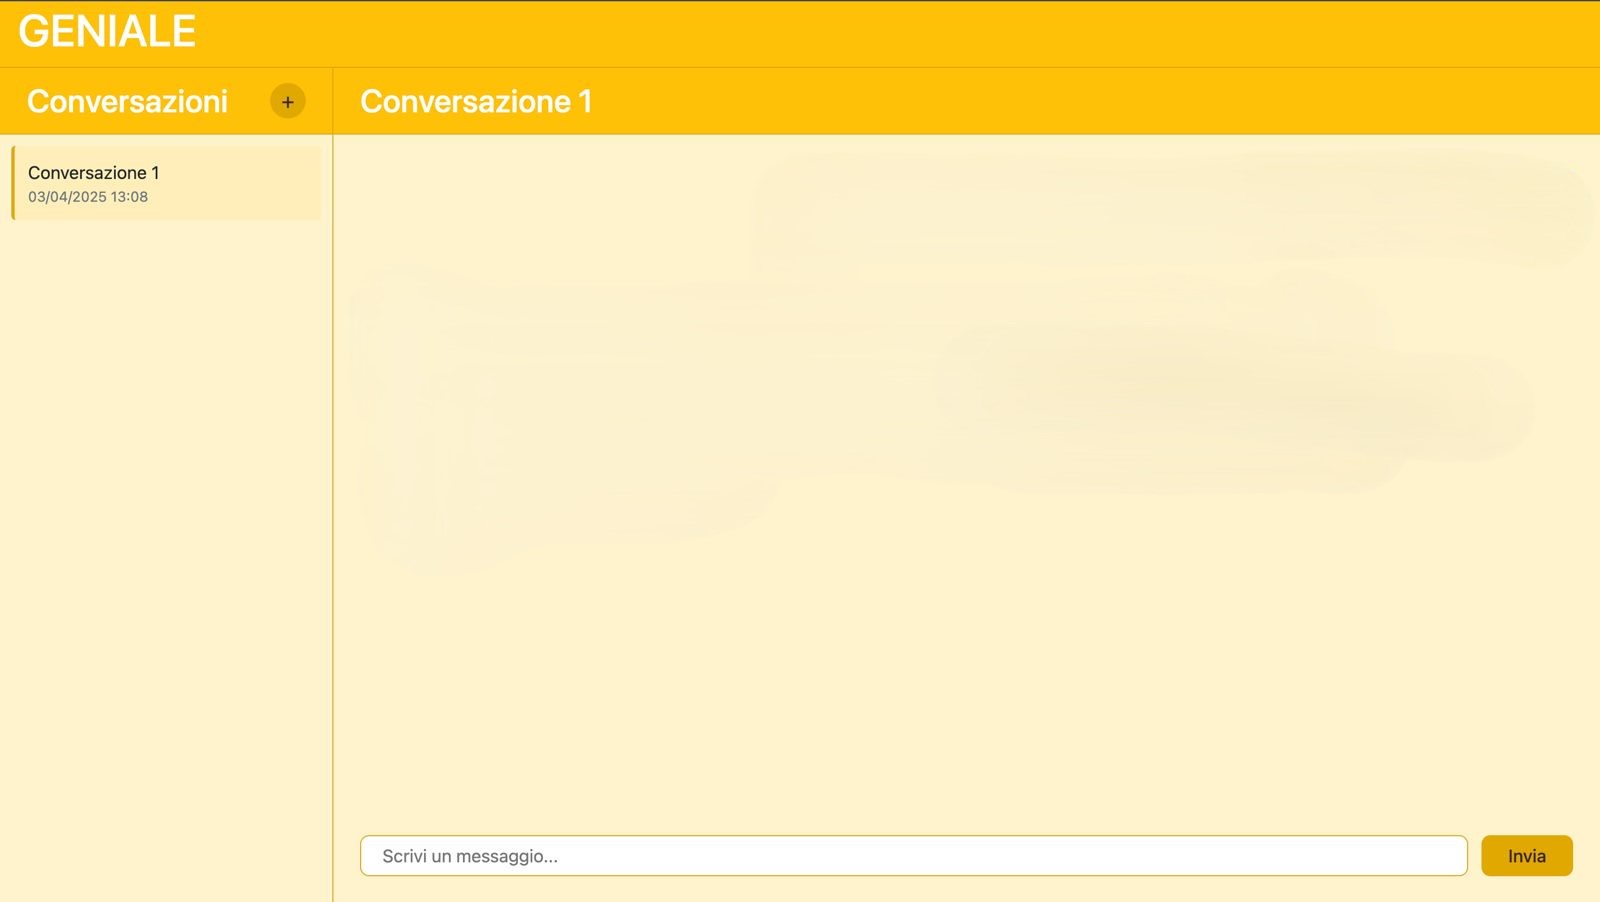
\includegraphics[width=1\textwidth]{contents/img/default_pc.jpg}
\caption{Interfaccia grafica al momento dell'avvio dell'applicativo}
\end{figure}

\subsubsection{Lista delle conversazioni}
\subsubsubsection{Convenzione per i nomi delle conversazioni}
Il titolo di ogni conversazione viene generato automaticamente ed è composto dalla parola "Conversazione", seguita da un identificativo univoco assegnato nel \textit{database}\textsubscript{G}. Questo permette di distinguere facilmente le diverse conversazioni create all'interno dell'applicazione.
\begin{figure}[H]
\centering
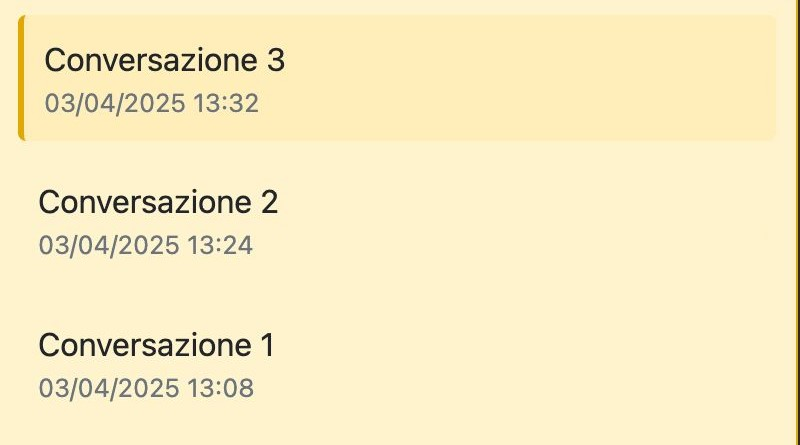
\includegraphics[width=1\textwidth]{contents/img/nome_conv.jpg}
\caption{Esempio di nomi assegnati alle conversazioni}
\end{figure}

\subsubsubsection{Comportamento di default}
Nel caso in cui non siano ancora presenti conversazioni, il \textit{sistema}\textsubscript{G} crea automaticamente una conversazione predefinita, in modo da garantire sempre un punto di partenza per l’utente.
\begin{figure}[H]
\centering

\includegraphics[width=1\textwidth]{contents/img/default_conv.jpg}
\caption{Creazione di una conversazione vuota in assenza di altre}
\end{figure}

\subsubsubsection{Visualizzazione della conversazione attiva}
Un altro dettaglio importante da notare è la modalità con cui viene evidenziata la conversazione attualmente aperta. Ad esempio, se nella sidebar è presente una chat denominata "Conversazione 3" con uno stile grafico differente rispetto alle altre, ciò indica che l’utente sta visualizzando proprio quella conversazione in quel momento. Questa rappresentazione visiva aiuta a orientarsi all’interno dell’elenco e a distinguere facilmente quale conversazione è attiva rispetto alle altre archiviate o meno recenti.
\begin{figure}[H]
\centering

\includegraphics[width=1\textwidth]{contents/img/active_conv.jpg}
\caption{Visualizzazione della conversazione attiva}
\end{figure}

\subsubsubsection{Creazione di nuove conversazioni}
Se si desidera avviare una nuova conversazione, è sufficiente selezionare il pulsante "+" posizionato accanto alla voce "Conversazioni" nella sidebar. Questo permette di generare una nuova istanza di chat, che verrà automaticamente aggiunta all'elenco e ordinata in base all'ultimo utilizzo.
\begin{figure}[H]
\centering

\includegraphics[width=1\textwidth]{contents/img/add_conv.jpg}
\caption{Pulsante per la creazione di nuove conversazioni}
\end{figure}

\subsubsubsection{Limite al numero di conversazioni disponibili}
Nel caso in cui l’utente raggiunga il numero massimo di conversazioni consentite, il \textit{sistema}\textsubscript{G} adotta un meccanismo di gestione intelligente per evitare il superamento di tale soglia. \\
Quando si tenta di creare una nuova conversazione oltre il limite previsto, compare un avviso (alert) che informa chiaramente l’utente della situazione. Il messaggio specifica che, procedendo con la creazione di una nuova conversazione, verrà eliminata automaticamente l’ultima conversazione nella lista, ovvero quella modificata meno di recente. Questo criterio si basa sull’ordine di utilizzo, non sul numero identificativo, quindi la conversazione che verrà rimossa è quella che non è stata aggiornata o aperta per più tempo. \\
L’alert non esegue l’azione in automatico, ma offre all’utente una scelta consapevole:
\begin{itemize}
    \item Proseguire comunque con la creazione della nuova conversazione, accettando la perdita di quella meno recente;
    \item Annullare l’operazione, in modo da poter eventualmente gestire manualmente le conversazioni esistenti, ad esempio eliminando una chat specifica o rivedendone i contenuti.
\end{itemize}
\begin{figure}[H]
\centering
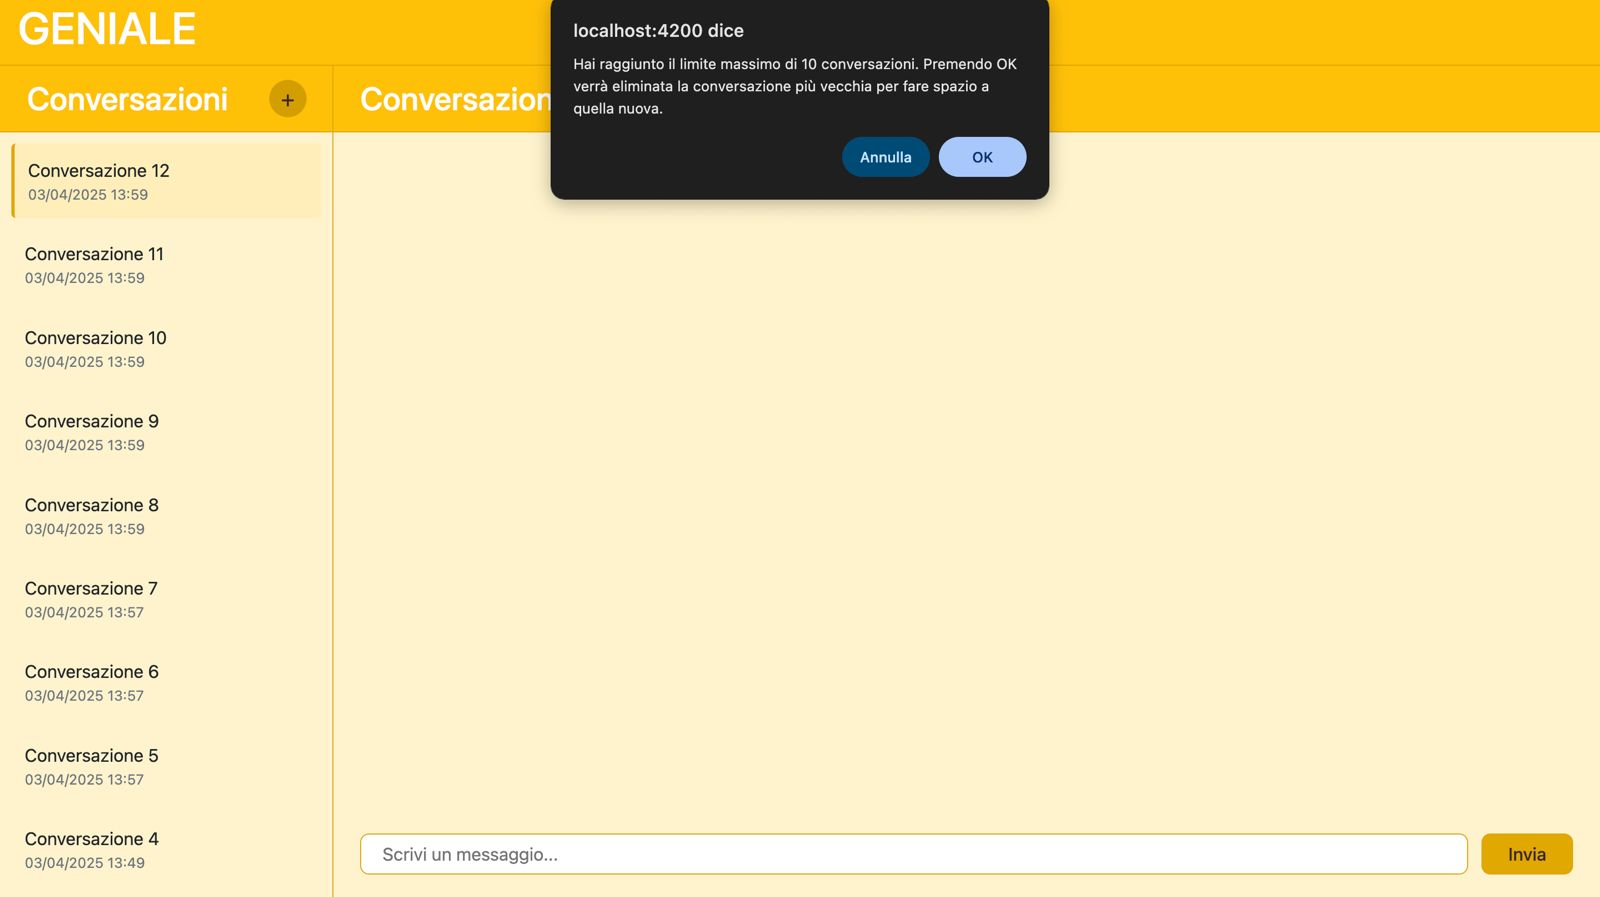
\includegraphics[width=1\textwidth]{contents/img/max_conv.jpg}
\caption{Alert che avvisa del raggiungimento del massimo numero di conversazioni}
\end{figure}

\subsubsubsection{Ordinamento delle conversazioni}
Nella sidebar, l’ordine delle conversazioni non segue il loro identificativo numerico (ovvero il numero che appare accanto alla parola “Conversazione”), ma è determinato dalla data e dall’ora dell’ultimo utilizzo. Questo valore, visibile sotto il titolo di ciascuna conversazione, corrisponde esattamente alla data e all’ora dell’ultimo messaggio ricevuto in quella chat. In questo modo, le conversazioni utilizzate più di recente vengono automaticamente posizionate in alto nella lista, garantendo un accesso rapido a quelle più attive.
\begin{figure}[H]
\centering
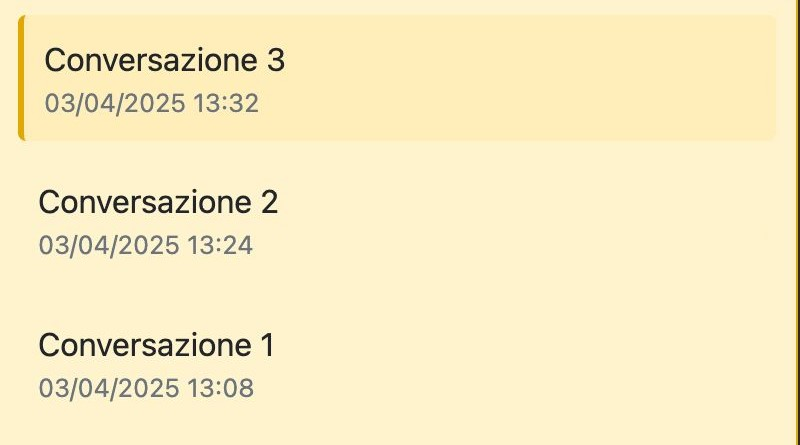
\includegraphics[width=1\textwidth]{contents/img/order_conv.jpg}
\caption{Esempio di ordinamento delle conversazioni}
\end{figure}

\subsubsubsection{Cancellazione di conversazioni}
Per eliminare una conversazione, l’utente può semplicemente cliccare sull’icona a forma di ‘x’ di colore rosso, posizionata accanto al titolo della conversazione desiderata all’interno della Sidebar. Questa funzione consente di rimuovere rapidamente e in modo intuitivo le conversazioni non più necessarie.
\begin{figure}[H]
\centering

\includegraphics[width=1\textwidth]{contents/img/rm_conv.jpg}
\caption{Pulsante per la creazione di nuove conversazioni}
\end{figure}
Se la conversazione selezionata per l’eliminazione non è quella attualmente visualizzata nella Chatbox, allora viene semplicemente rimossa dalla Sidebar, senza alcun impatto sulla schermata principale. L’utente può continuare a interagire con la conversazione aperta senza interruzioni o modifiche al contenuto.
\begin{figure}[H]
\centering
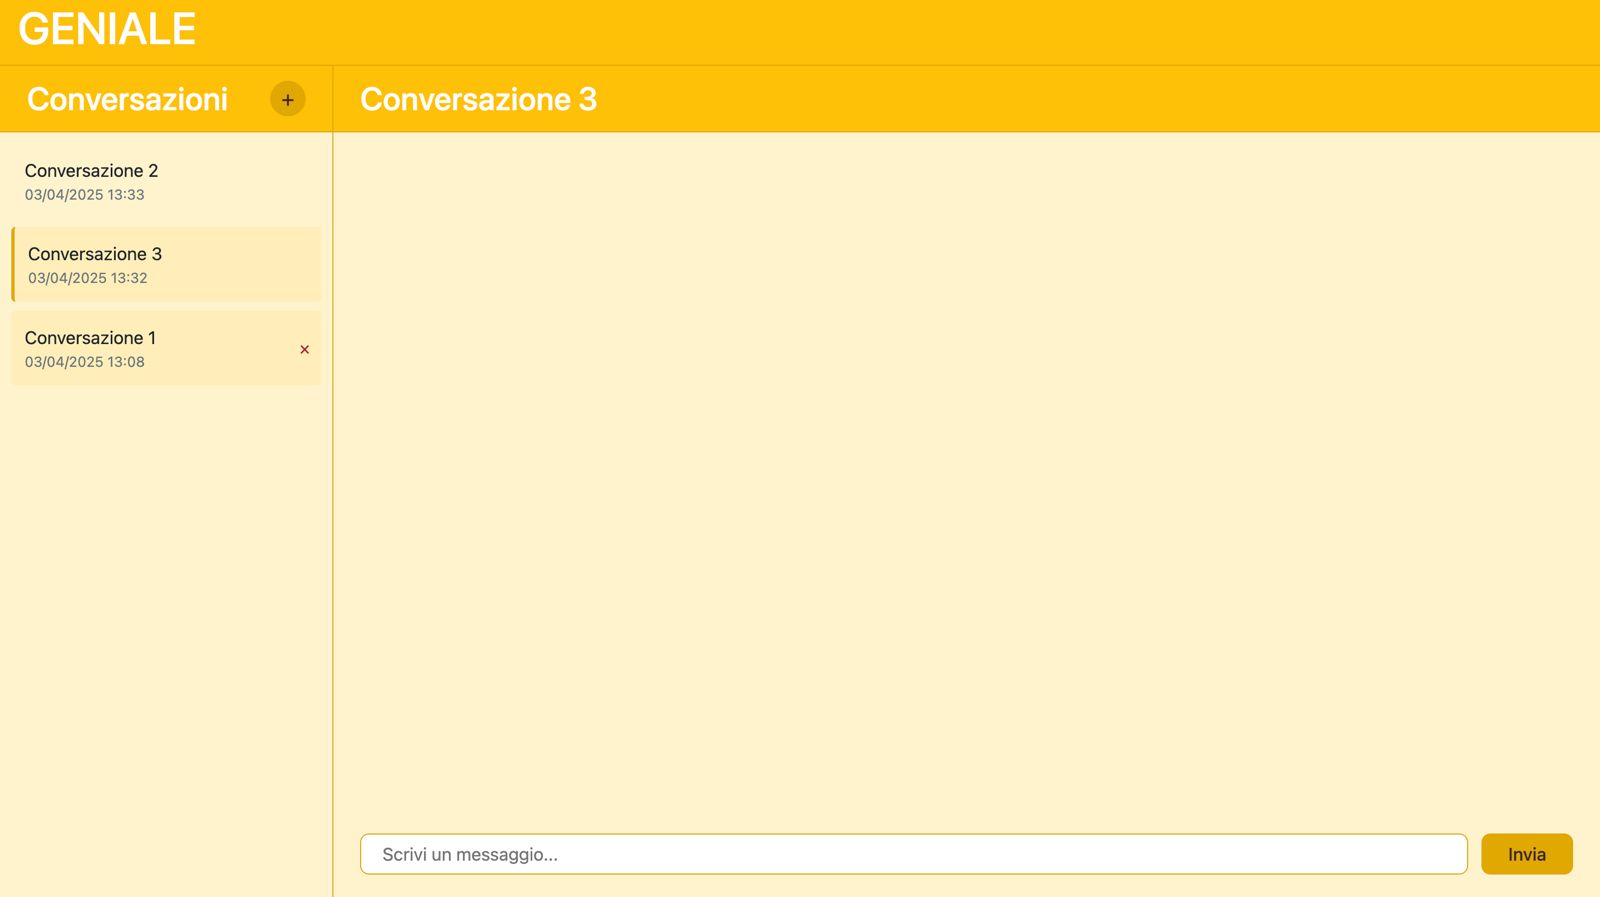
\includegraphics[width=1\textwidth]{contents/img/rm_conv_inactive_before.jpg}
\caption{Situazione prima della cancellazione di una conversazione inattiva}
\end{figure}
\begin{figure}[H]
\centering
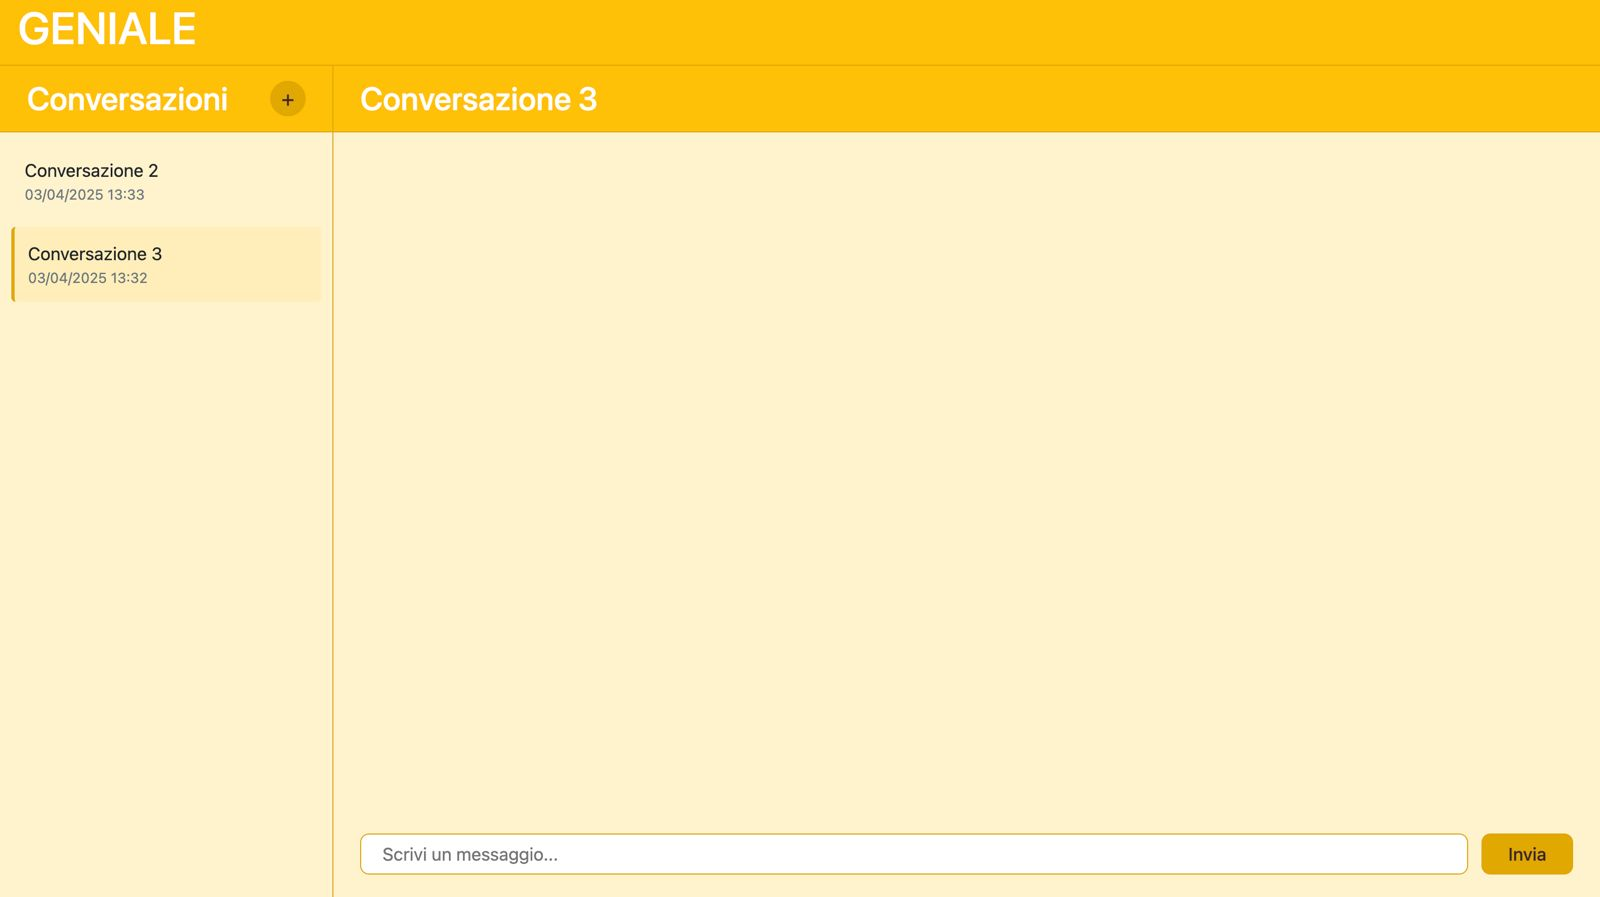
\includegraphics[width=1\textwidth]{contents/img/rm_conv_inactive_after.jpg}
\caption{Situazione dopo la cancellazione di una conversazione inattiva}
\end{figure}
Nel caso in cui l’utente elimini la conversazione attualmente attiva, l’interfaccia si aggiorna immediatamente: al posto della conversazione eliminata viene creata automaticamente una nuova conversazione di default. Questa nuova conversazione viene caricata nella Chatbox e contrassegnata come attiva, garantendo così la continuità dell’esperienza d’uso. In questo modo, l’utente non si ritrova mai senza una conversazione aperta e può proseguire immediatamente con una nuova interazione.
\begin{figure}[H]
\centering
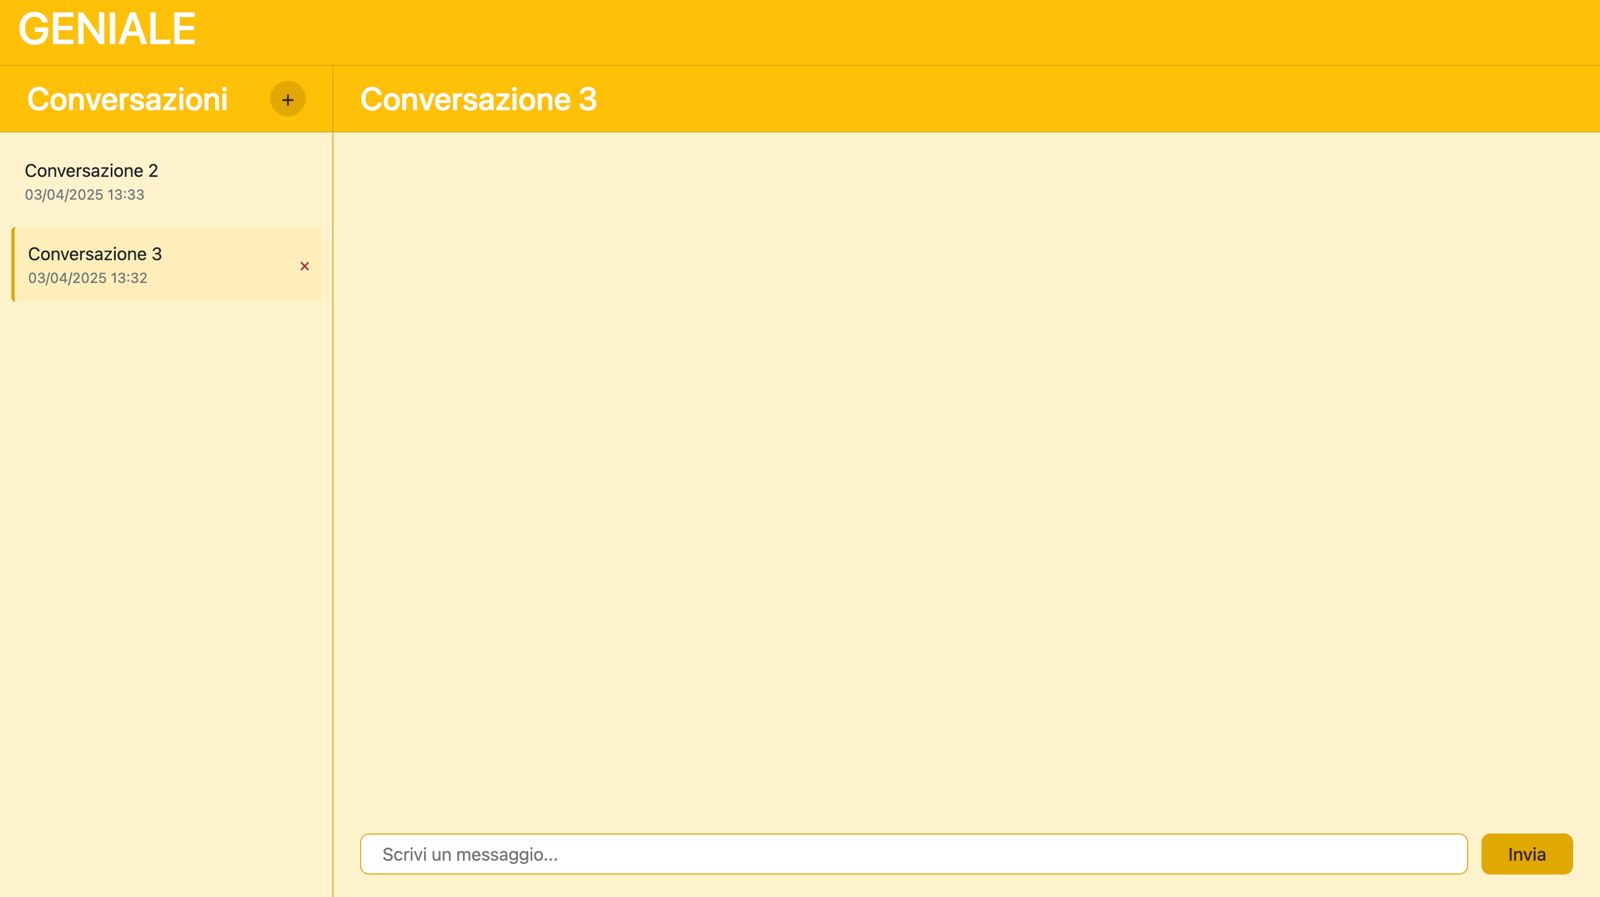
\includegraphics[width=1\textwidth]{contents/img/rm_conv_active_before.jpg}
\caption{Situazione prima della cancellazione della conversazione attiva}
\end{figure}
\begin{figure}[H]
\centering
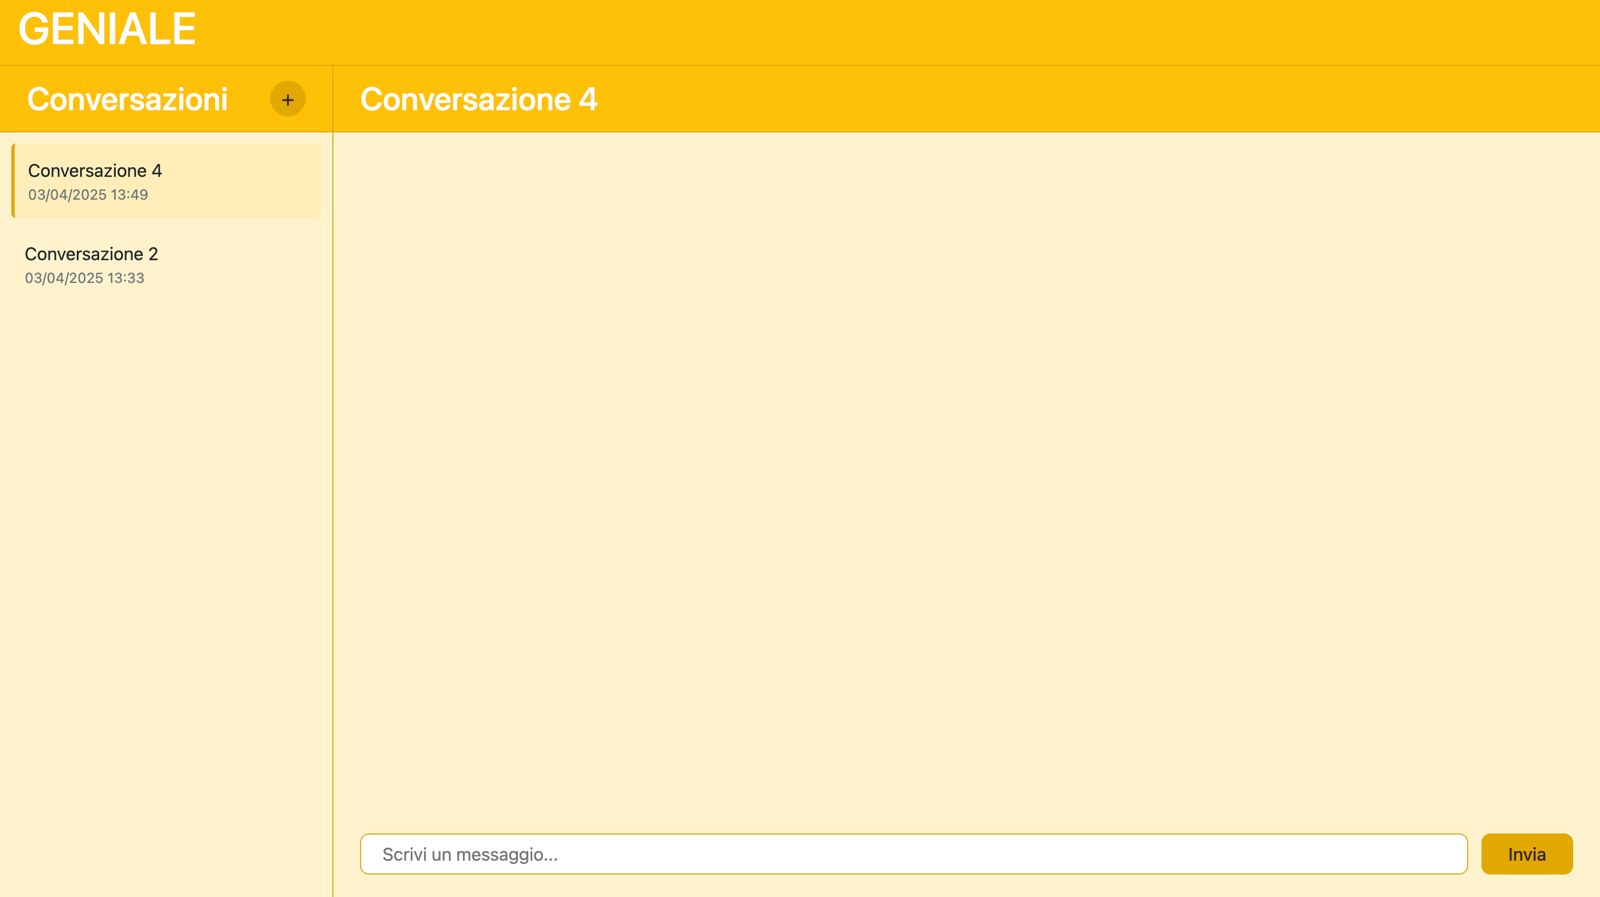
\includegraphics[width=1\textwidth]{contents/img/rm_conv_active_after.jpg}
\caption{Situazione dopo la cancellazione della conversazione attiva}
\end{figure}

\subsubsection{Conversazione attiva}
\subsubsubsection{Inserimento e invio della domanda}
Nell’interfaccia, l’inserimento della domanda da parte dell’utente avviene tramite un campo di testo posizionato nella parte inferiore della schermata. Questo box, ben visibile e facilmente accessibile, presenta la dicitura “Scrivi un messaggio...”, che funge da indicazione chiara e intuitiva sull’uso dell’elemento. \\
Alla destra del campo di \textit{input}\textsubscript{G} è presente il pulsante “Invia”, evidenziato da uno sfondo giallo scuro, che consente di trasmettere il messaggio al \textit{sistema}\textsubscript{G}. Una volta premuto, il contenuto viene inviato all’assistente digitale, che risponde visualizzando il messaggio all’interno della conversazione, seguendo un ordinamento cronologico domanda-risposta. \\
È importante notare che, per garantire un funzionamento corretto del \textit{sistema}\textsubscript{G}, è previsto un limite alla lunghezza del testo inseribile. Questo limite serve a mantenere l’esperienza utente fluida e a favorire risposte più rapide e coerenti.
\begin{figure}[H]
\centering
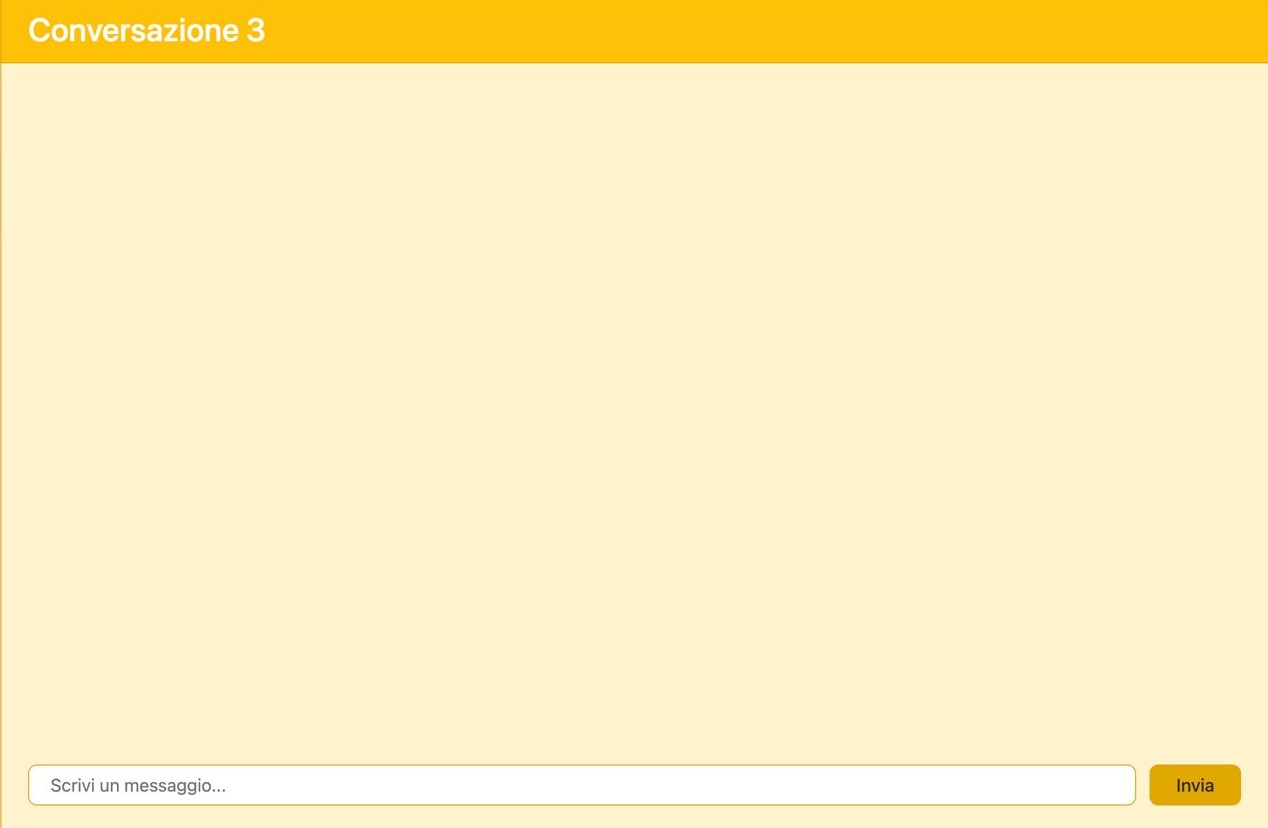
\includegraphics[width=1\textwidth]{contents/img/conv_pc.jpg}
\caption{Interfaccia per l'inserimento e l'invio della domanda}
\end{figure}

\subsubsubsection{Blocco delle funzionalità dopo la domanda}
Durante il processo di invio di un messaggio, l’applicazione impone una limitazione temporanea delle interazioni, assicurandosi che venga prima ricevuta la risposta dell’assistente digitale prima di consentire nuove azioni. Questo meccanismo è progettato per garantire che la generazione della risposta avvenga senza interruzioni o anomalie, migliorando la stabilità e l’affidabilità dell’esperienza utente. \\
Dal punto di vista dell’interfaccia grafica, questa limitazione si traduce in una serie di blocchi momentanei sulle funzionalità dell’applicazione. Nello specifico:
\begin{itemize}
    \item Non è possibile creare nuove conversazioni utilizzando il pulsante “+” accanto alla voce “Conversazioni” nella sidebar;
    \item Non si possono selezionare altre conversazioni presenti nella sidebar, impedendo così all’utente di passare da una chat all’altra mentre è in attesa di una risposta;
    \item Non si possono inviare nuovi messaggi, evitando che l’utente sovrapponga richieste mentre l’assistente è ancora in elaborazione.
\end{itemize}
Durante questa fase di attesa, l’interfaccia mostra un indicatore visivo: al posto della risposta dell’assistente compare la scritta "Sto pensando..." accompagnata da uno spinner animato, segnalando che il \textit{sistema}\textsubscript{G} è in fase di elaborazione. Solo quando questo testo scompare e viene visualizzata la risposta generata dall’assistente digitale, le funzionalità dell’applicazione vengono ripristinate, consentendo nuovamente l’invio di messaggi e l’interazione con la sidebar.
\begin{figure}[H]
\centering
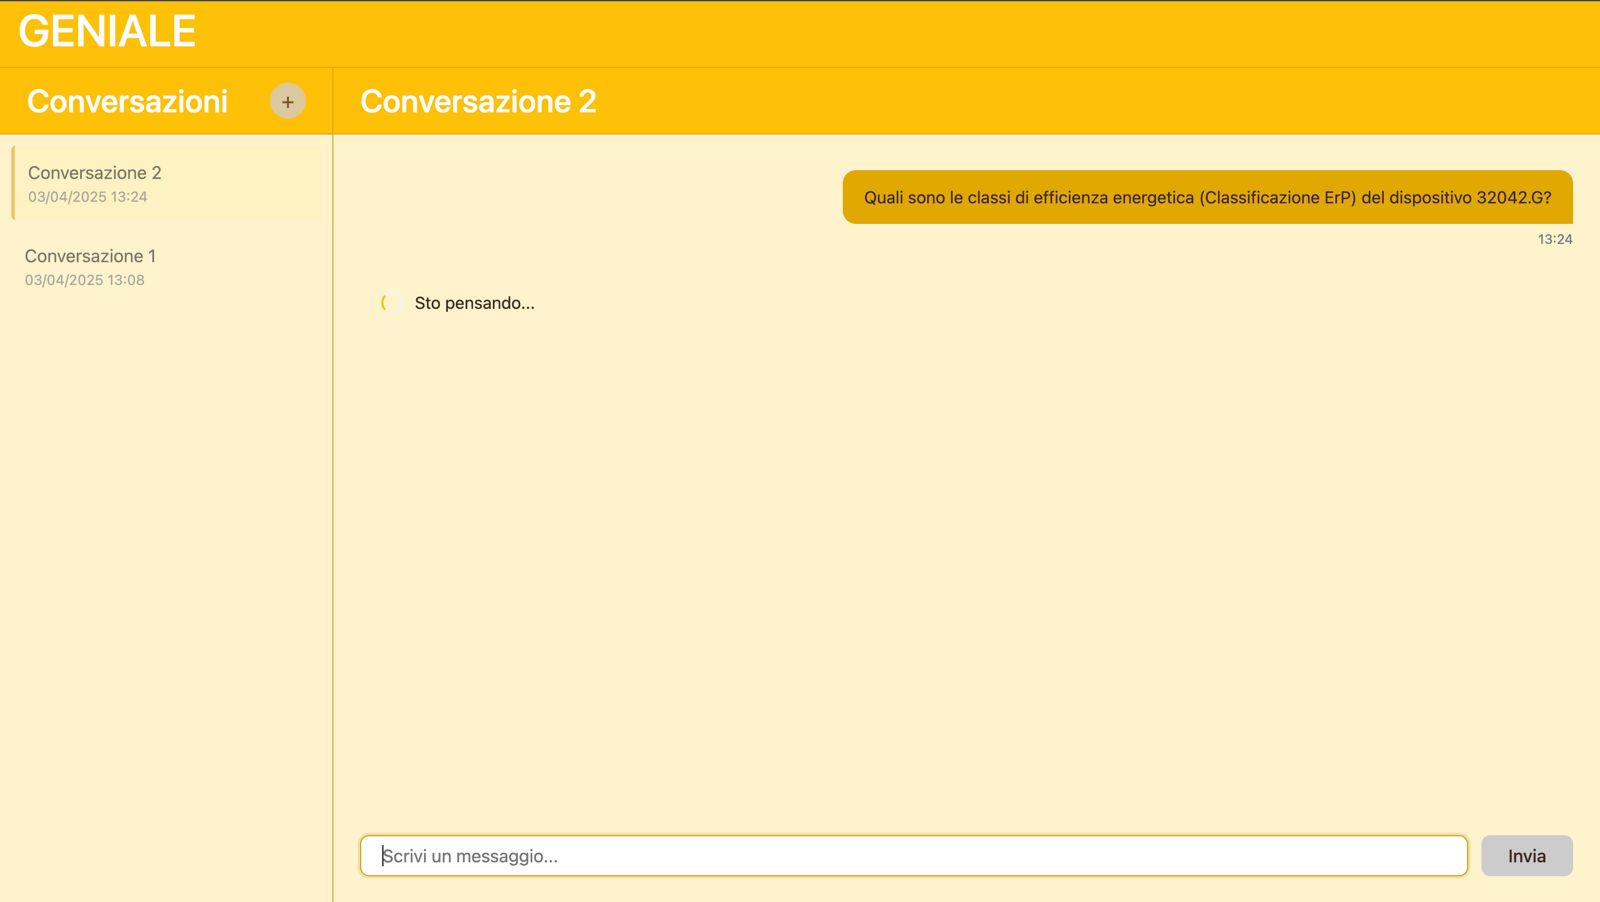
\includegraphics[width=1\textwidth]{contents/img/lock_pc.jpg}
\caption{Limitazione delle interazioni durante l'attensa di una risposta}
\end{figure}

\subsubsubsection{Sistema di feedback}
Come si può osservare dall’interfaccia, ogni messaggio ricevuto dall’assistente digitale è accompagnato non solo dall’orario di ricezione, ma anche da un \textit{sistema}\textsubscript{G} di \textit{feedback}\textsubscript{G} visivo che consente all’utente di esprimere una valutazione immediata sulla qualità o l’utilità della risposta ricevuta. \\
Questo \textit{sistema}\textsubscript{G} si basa su due icone intuitive e facilmente riconoscibili:
\begin{itemize}
    \item Il pollice in su, contrassegnato dal colore verde, indica un \textit{feedback}\textsubscript{G} positivo. Selezionando questa opzione, l’utente comunica che la risposta è stata soddisfacente, utile o corretta;
    \item Il pollice in giù, contrassegnato dal colore rosso, rappresenta invece un \textit{feedback}\textsubscript{G} negativo, attraverso il quale l’utente segnala che la risposta non è stata utile, è risultata incompleta, imprecisa o fuori contesto.
\end{itemize}
\begin{figure}[H]
\centering
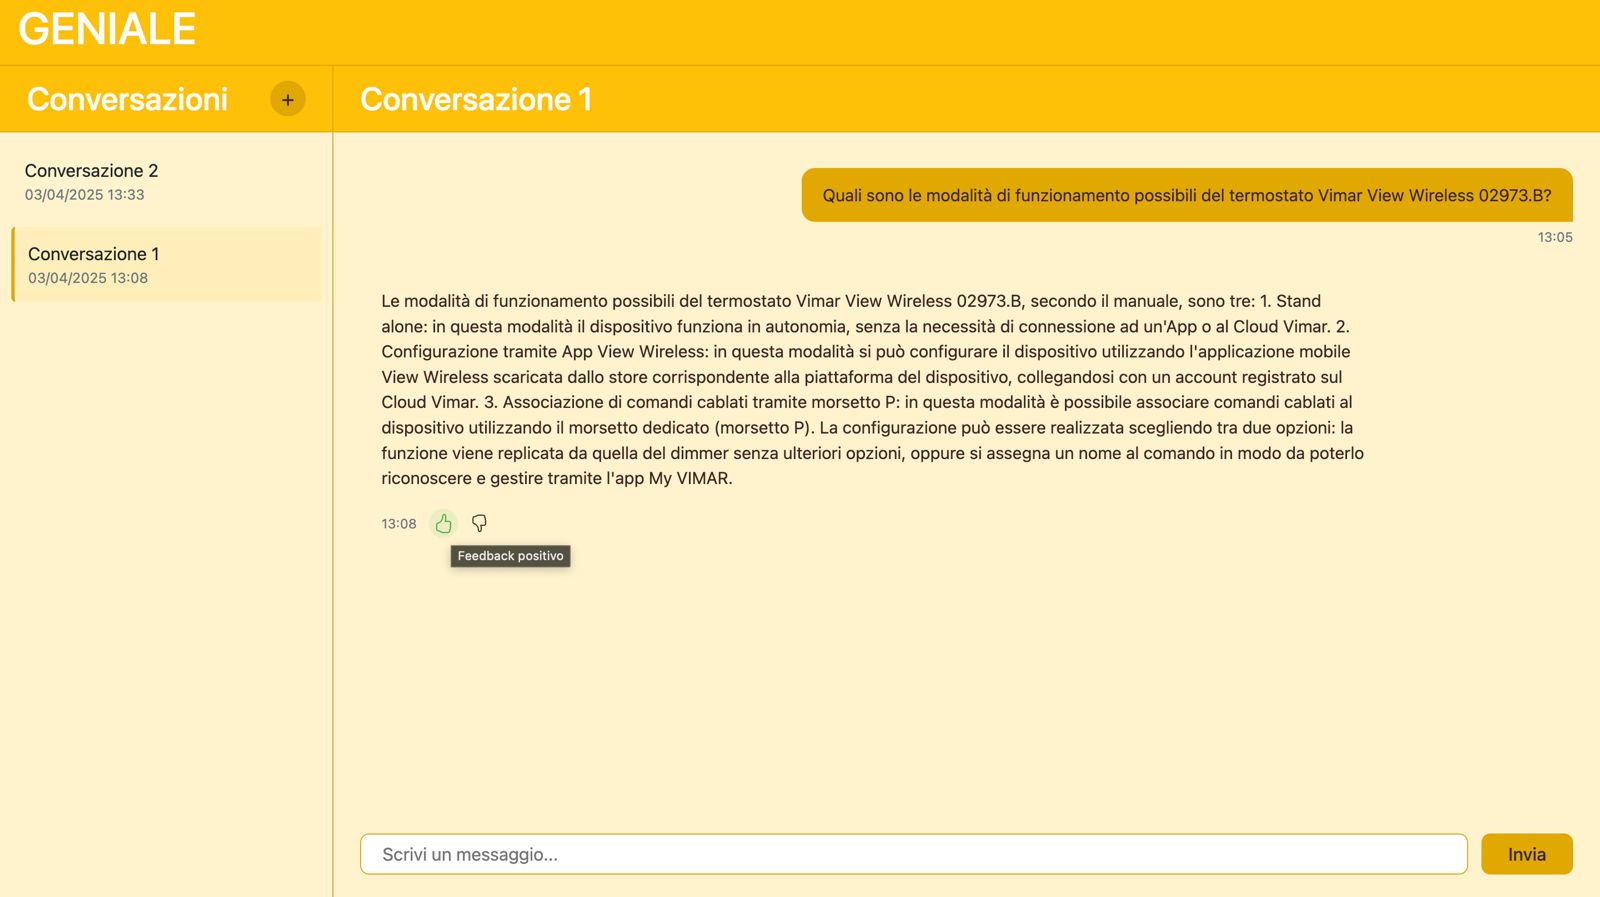
\includegraphics[width=1\textwidth]{contents/img/feedback.jpg}
\caption{Pulsanti per fornire il \textit{feedback}\textsubscript{G} relativo ad una risposta}
\end{figure}
Quando l’utente seleziona uno di questi due pulsanti si attiva un pop-up di conferma che consente di fornire un commento facoltativo a supporto della valutazione espressa. \\
All’interno di questo pop-up, l’utente ha due possibilità:
\begin{itemize}
    \item Inviare il \textit{feedback}\textsubscript{G} senza aggiungere alcun commento, limitandosi a confermare la valutazione tramite l’icona selezionata;
    \item Scrivere un commento descrittivo o contestuale per spiegare meglio il motivo del giudizio positivo o negativo.
\end{itemize}
\begin{figure}[H]
\centering
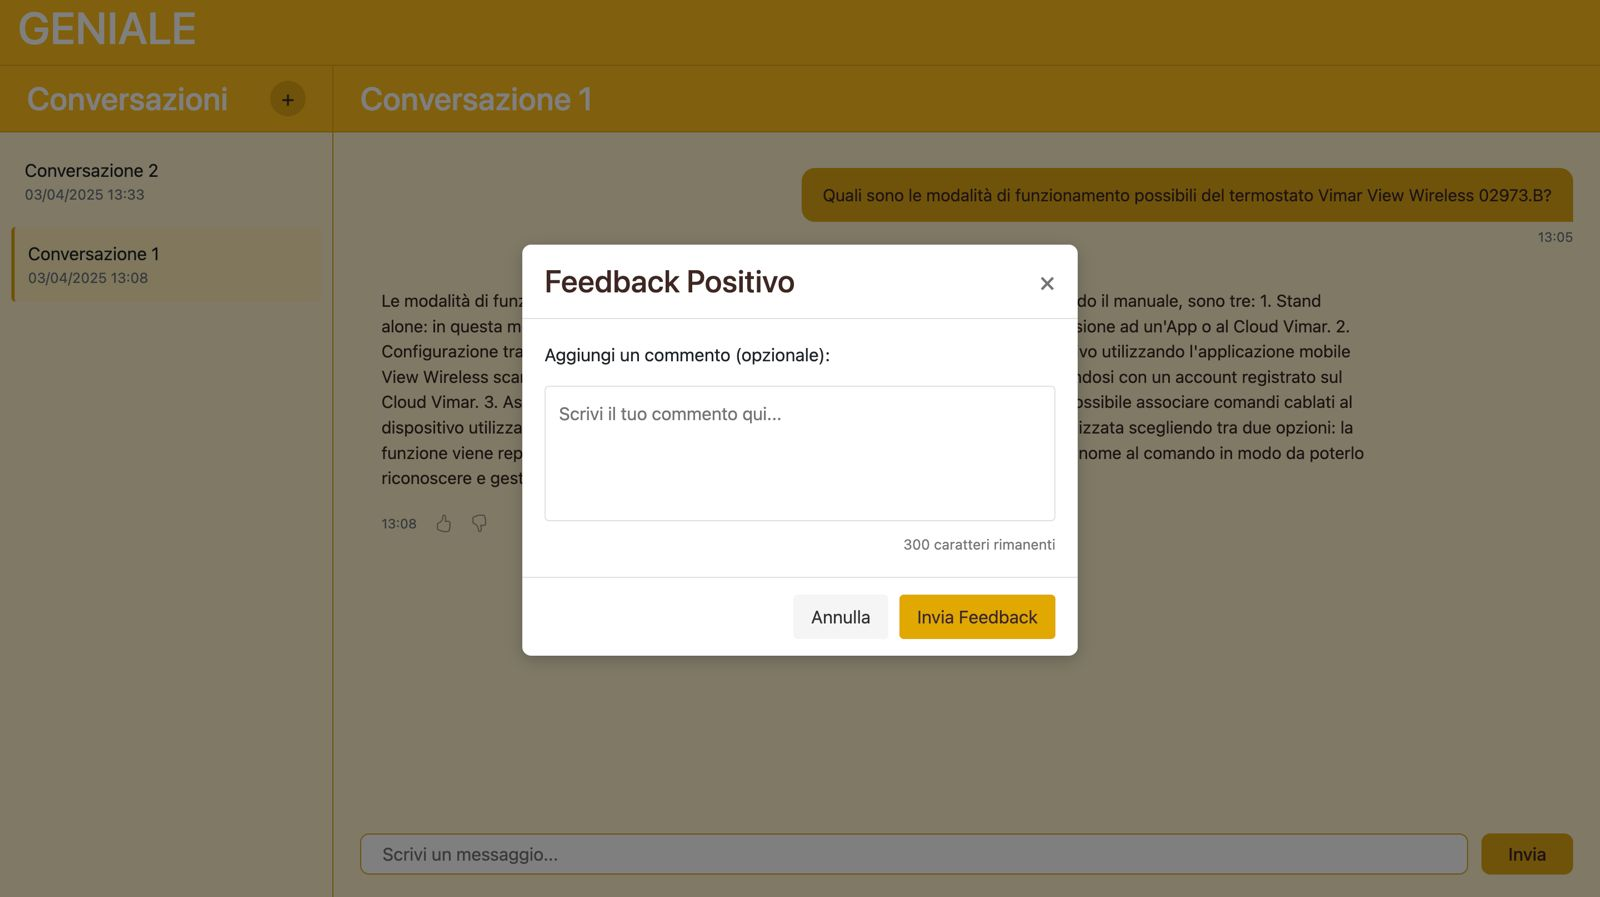
\includegraphics[width=1\textwidth]{contents/img/feedback_comment.jpg}
\caption{Pop-up che consente l'inserimento di un commento aggiuntivo al \textit{feedback}\textsubscript{G}}
\end{figure}
Una volta che l’utente invia un \textit{feedback}\textsubscript{G} relativo a un messaggio dell’assistente digitale, l’interfaccia dell’applicativo si aggiorna per contrassegnare visivamente quel messaggio con il tipo di \textit{feedback}\textsubscript{G} selezionato. \\
Il messaggio viene quindi marcato in modo chiaro con l’icona corrispondente:
\begin{itemize}
    \item Il pollice in su verde, se è stato fornito un \textit{feedback}\textsubscript{G} positivo;
    \item Il pollice in giù rosso, se è stato fornito un \textit{feedback}\textsubscript{G} negativo.
\end{itemize}
Questa marcatura resta permanente e visibile, fungendo sia da conferma per l’utente che da riferimento per eventuali revisioni future da parte del team di sviluppo. È importante sottolineare che il \textit{feedback}\textsubscript{G}, una volta inviato, non può essere modificato. Non è possibile né cambiare la valutazione data né inviarne una nuova per lo stesso messaggio.
\begin{figure}[H]
\centering
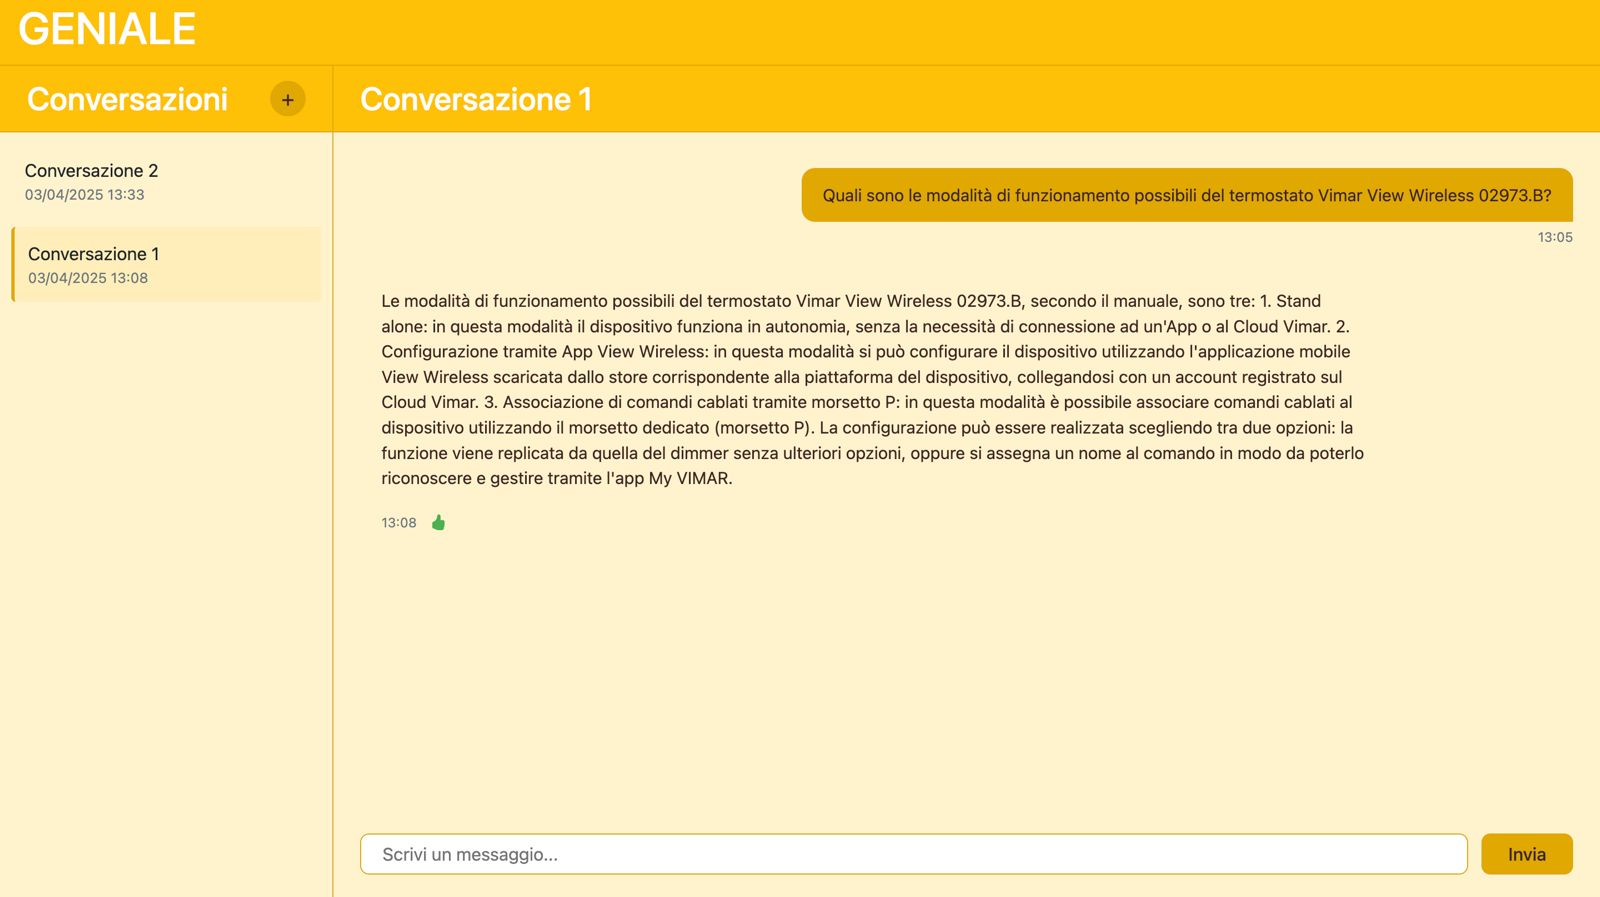
\includegraphics[width=1\textwidth]{contents/img/feedback_result.jpg}
\caption{Aggiornamento dell'interfaccia dopo l'invio di un \textit{feedback}\textsubscript{G}}
\end{figure}
Questo meccanismo di valutazione è pensato per essere immediato, discreto e non invasivo, offrendo un modo semplice per raccogliere indicazioni sulla qualità delle risposte dell’assistente. Inoltre, permette al \textit{sistema}\textsubscript{G} di migliorare progressivamente le proprie prestazioni, tenendo conto delle valutazioni fornite dagli utenti nel tempo.

\subsubsection{Area riservata per gli amministratori}
\'E importante sottolineare che la sezione amministrativa dell’applicativo è accessibile in modo diretto tramite una modifica dell’URL utilizzato normalmente dagli utenti generici. \\
Per accedervi, è sufficiente aggiungere il segmento "/admin" alla fine dell’indirizzo URL principale dell’applicativo. Ad esempio, se l’URL standard per l’utente generico è \texttt{localhost:4200} basterà digitare \texttt{localhost:4200/admin} per essere reindirizzati all’interfaccia dedicata agli amministratori o sviluppatori.

\subsubsubsection{Login}
L’area riservata all’\textit{Amministratore}\textsubscript{G} dell’applicativo è protetta da un \textit{sistema}\textsubscript{G} di autenticazione, pensato per garantire la sicurezza e impedire l’accesso non autorizzato a funzionalità sensibili. \\
Per accedervi, è necessario inserire una \textit{password}\textsubscript{G} valida nella schermata di login che compare automaticamente quando si tenta di raggiungere l’URL dell’area amministrativa (aggiungendo, ad esempio, "/admin" all’indirizzo principale dell’applicativo). Solo gli utenti autorizzati, in possesso delle credenziali corrette, possono superare questa fase di autenticazione.
\begin{figure}[H]
\centering
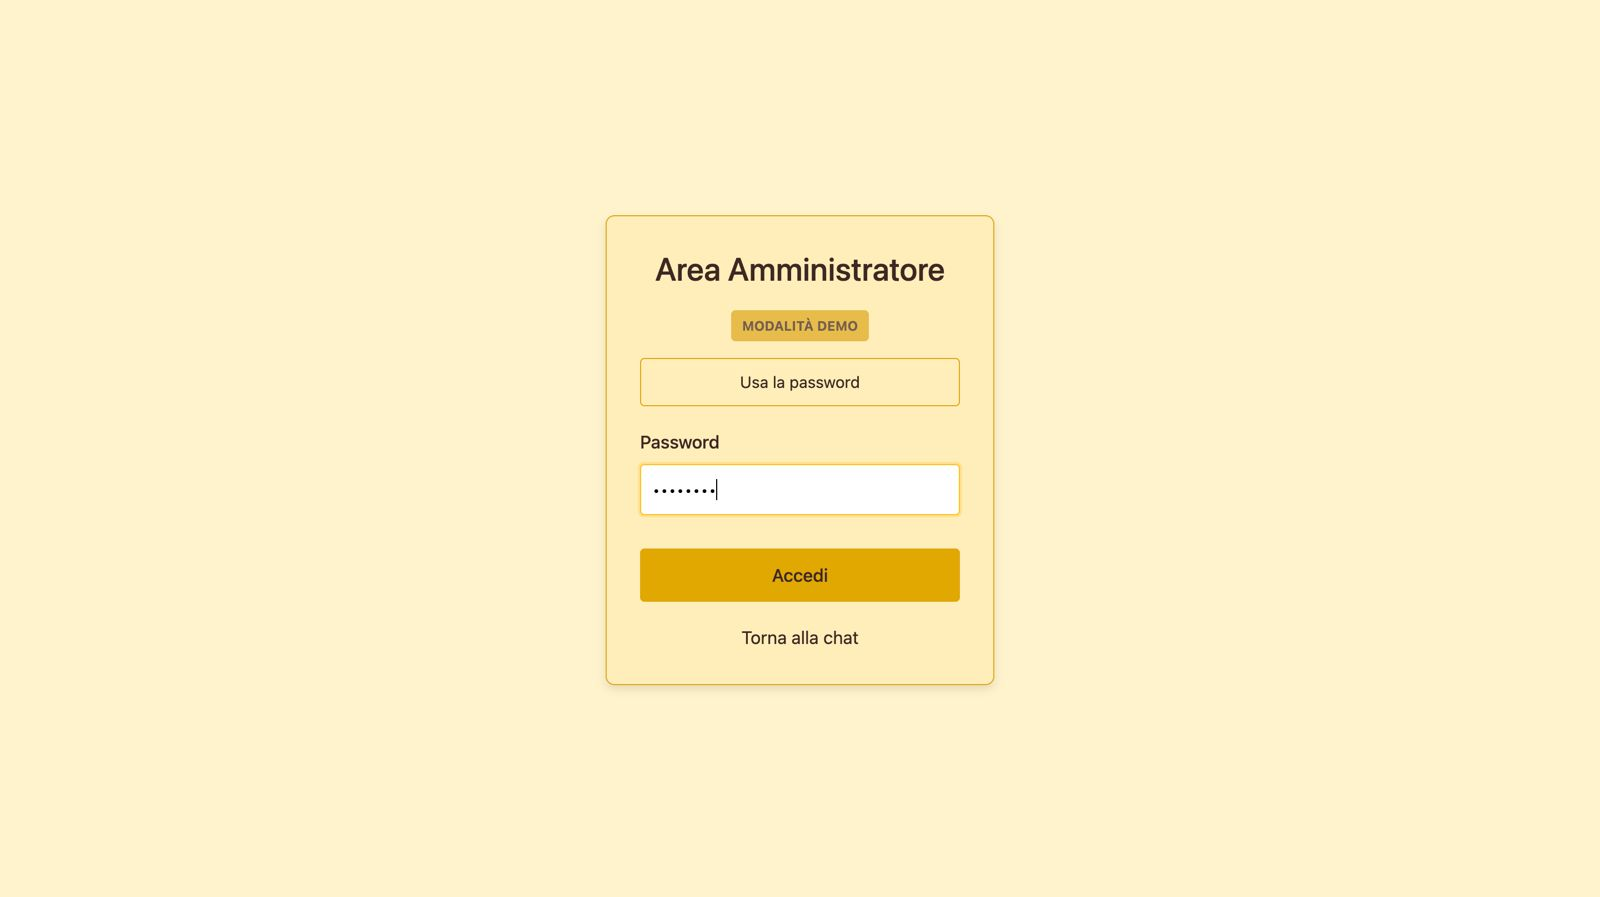
\includegraphics[width=1\textwidth]{contents/img/login.jpg}
\caption{Schermata di login per accedere alla \textit{dashboard}\textsubscript{G} per gli amministratori}
\end{figure}

\subsubsubsection{Dashboard per l'amministratore}
La \textit{dashboard}\textsubscript{G} per l'\textit{amministratore}\textsubscript{G} dell’applicativo fornisce una panoramica dettagliata e aggiornata sull’utilizzo del \textit{sistema}\textsubscript{G} da parte degli utenti, offrendo dati preziosi per il monitoraggio delle prestazioni e l’identificazione di aree di miglioramento. \\
Tra le principali informazioni visualizzabili nella \textit{dashboard}\textsubscript{G} si trovano:
\begin{itemize}
    \item Il numero totale di conversazioni avviate dagli utenti all’interno dell’applicativo;
    \item Il numero complessivo di \textit{feedback}\textsubscript{G} ricevuti, distinti tra positivi e negativi;
    \item Un tasso di soddisfazione complessivo, calcolato in base alla proporzione tra \textit{feedback}\textsubscript{G} positivi e negativi, che fornisce un’indicazione immediata sul livello di gradimento delle risposte generate dall’assistente digitale.
\end{itemize}
Oltre ai dati aggregati, la \textit{dashboard}\textsubscript{G} consente anche di visualizzare i feedback accompagnati da un commento testuale. Questi \textit{feedback}\textsubscript{G} “non vuoti” sono particolarmente utili per il team di sviluppo, in quanto offrono spunti concreti e specifici per il miglioramento dell’algoritmo, dell’interfaccia o della qualità delle risposte. \\
Per quanto riguarda le azioni disponibili all’interno di questa sezione riservata, l’\textit{amministratore}\textsubscript{G} può scegliere tra due opzioni:
\begin{itemize}
    \item \textbf{Logout}: Selezionando questa opzione, per accedere nuovamente all’area amministrativa, sarà necessario ripetere il processo di autenticazione;
    \item \textbf{Torna alla chat}: Questa opzione permette di ritornare all’interfaccia utente standard, quella dedicata alle conversazioni, senza disconnettersi, e quindi l’\textit{amministratore}\textsubscript{G} potrà accedere nuovamente alla \textit{dashboard}\textsubscript{G} in qualsiasi momento, senza dover reinserire la \textit{password}\textsubscript{G}, fino a quando non esegue un logout esplicito o svuota manualmente la memoria locale del browser.
\end{itemize}
\begin{figure}[H]
\centering
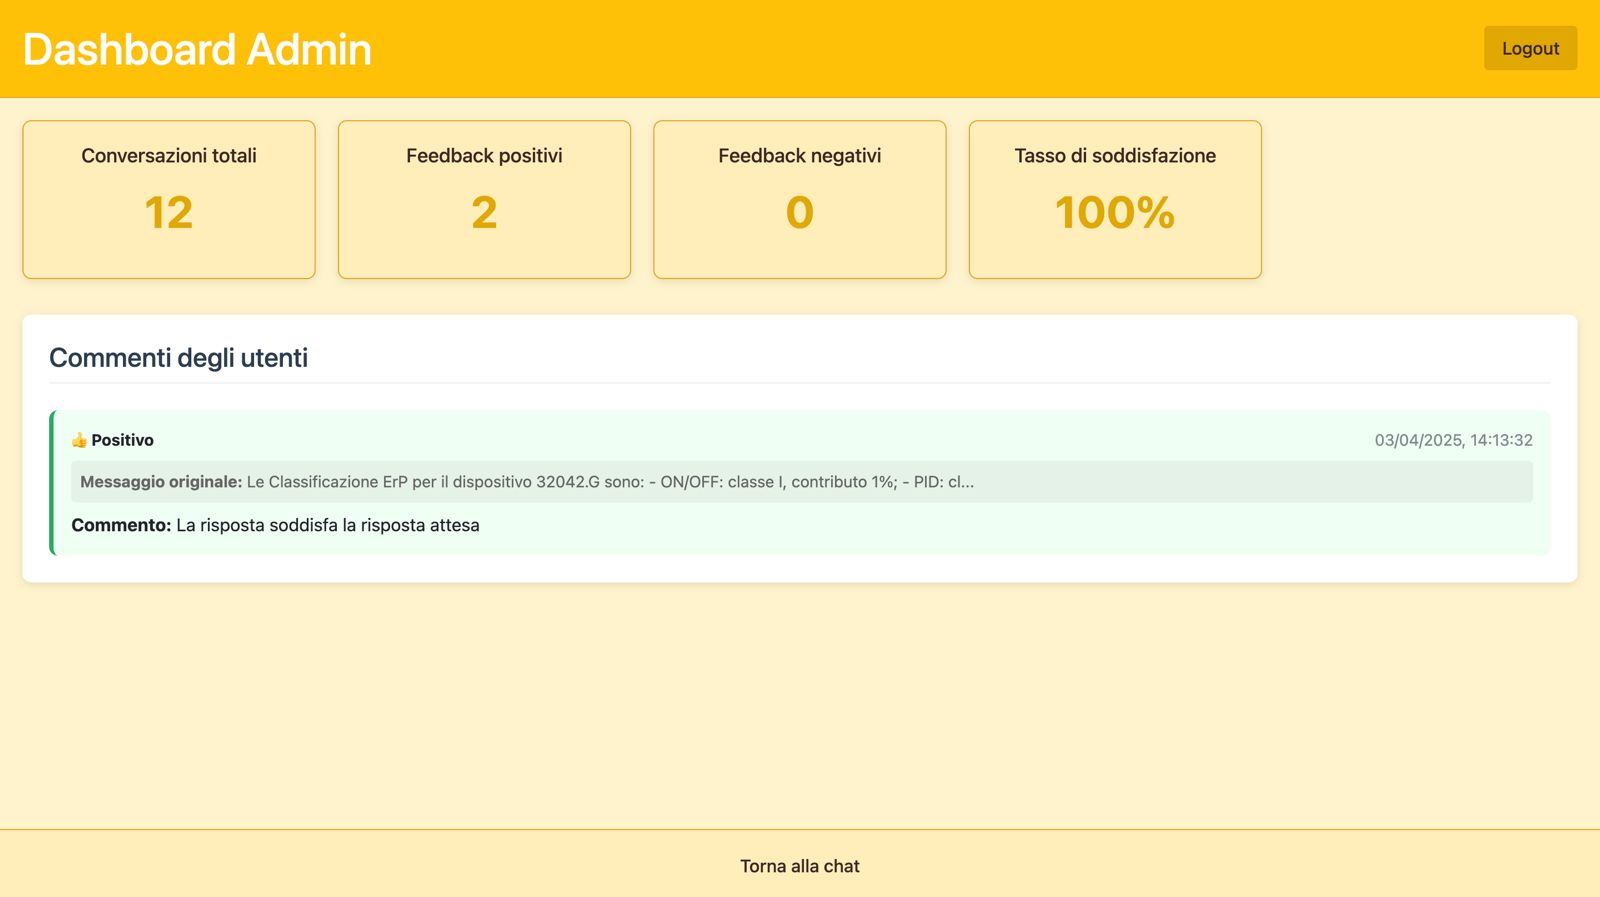
\includegraphics[width=1\textwidth]{contents/img/dashboard.jpg}
\caption{\textit{dashboard}\textsubscript{G} per gli amministratori}
\end{figure}

\subsection{Versione mobile dell'applicativo}
Durante l’utilizzo dell’applicativo su dispositivi mobili o, più in generale, su schermi di dimensioni ridotte, l’interfaccia si adatta automaticamente per garantire una navigazione fluida e ordinata. \\
In questa modalità responsive, la schermata principale non mostra contemporaneamente sia la sidebar (contenente la lista delle conversazioni) sia la chatbox (l’area dedicata alla conversazione attiva), per ottimizzare lo spazio disponibile e migliorare la leggibilità dei contenuti. \\
La soluzione adottata permette di mantenere intatta la funzionalità dell’applicativo anche su schermi piccoli, offrendo all’utente un’esperienza coerente, intuitiva e facilmente navigabile, senza rinunciare a nessuna delle caratteristiche presenti nella versione desktop.\\
Di seguito verranno quindi riportate le caratteristiche che sono state aggiunte o che sono state modificate rispetto alla versione desktop.
\begin{figure}[H]
\centering
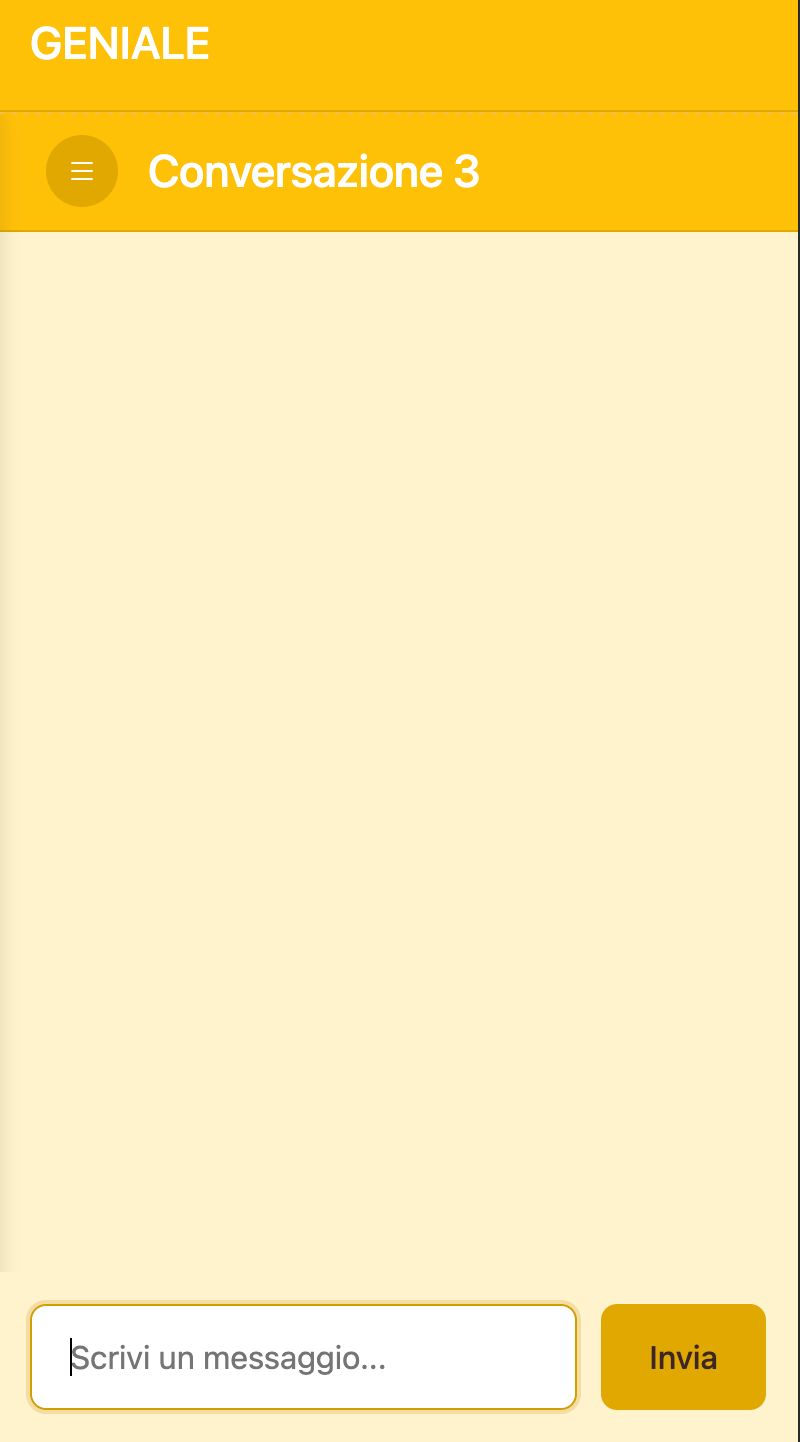
\includegraphics[width=0.5\textwidth]{contents/img/active_conv_mobile.jpg}
\caption{Interfaccia grafica al momento dell’avvio dell’applicativo}
\end{figure}

\subsubsection{Pulsante per visualizzare la lista di conversazioni}
Per ovviare alla limitazione visiva, compare un pulsante posizionato a sinistra del titolo della conversazione, che consente all’utente di accedere alla lista delle conversazioni. Questo pulsante è specifico per la visualizzazione mobile e appare solo quando la larghezza dello schermo è troppo ridotta per ospitare entrambe le sezioni dell’interfaccia affiancate. \\
Toccando il pulsante, l’utente può aprire la sidebar in modalità a comparsa (overlay o slide-in), visualizzare le conversazioni esistenti, selezionarne una diversa o crearne una nuova, per poi tornare alla chatbox con la conversazione selezionata.
\begin{figure}[H]
\centering

\includegraphics[width=1\textwidth]{contents/img/toggle.jpg}
\caption{Pulsante per visualizzare la lista di conversazioni disponibili}
\end{figure}

\subsubsection{Lista delle conversazioni disponibili}
Selezionando il pulsante di cui abbiamo appena discusso, l’utente può attivare la visualizzazione della Sidebar, la quale prende il posto della Chatbox principale. In questo modo, la lista delle conversazioni diventa pienamente visibile e navigabile, permettendo all’utente di consultare le chat esistenti o avviarne di nuove. \\
Una volta selezionata una conversazione già presente nell’elenco, oppure creandone una nuova tramite il pulsante “+”, la Sidebar si chiude automaticamente, lasciando nuovamente spazio alla Chatbox. Questo comportamento consente di mantenere il flusso della conversazione attivo e senza distrazioni, focalizzando l’attenzione dell’utente sulla chat attuale.
\begin{figure}[H]
\centering
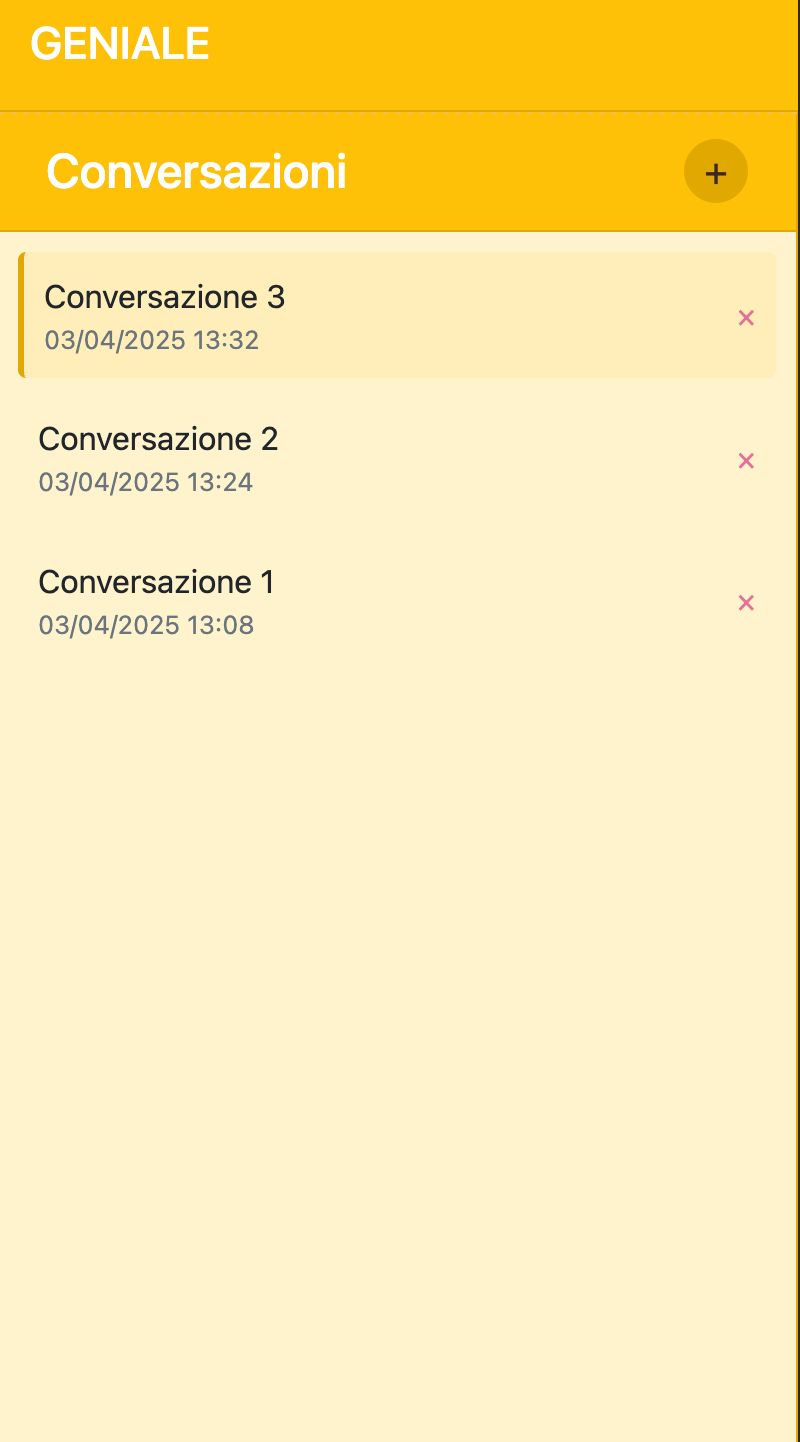
\includegraphics[width=0.5\textwidth]{contents/img/list_conv_mobile.jpg}
\caption{Visualizzazione di tutte le conversazione disponibili}
\end{figure}

\subsubsection{Blocco delle funzionalità dopo la domanda}
Anche nella versione mobile o su schermi ridotti, la logica di limitazione delle azioni durante la fase di elaborazione della risposta da parte dell’assistente digitale rimane attiva e coerente con quanto avviene nella versione desktop. Questo significa che, mentre il \textit{sistema}\textsubscript{G} è impegnato nella generazione di una risposta, tutte le funzionalità interattive principali dell’interfaccia vengono temporaneamente disabilitate, indipendentemente dal dispositivo utilizzato. In particolare:
\begin{itemize}
    \item La lista delle conversazioni non è accessibile: viene nascosta o resa non interattiva fino al completamento del processo di risposta;
    \item Non è possibile inviare nuovi messaggi: il campo di \textit{input}\textsubscript{G} viene disattivato e l’invio è bloccato fino a quando l’assistente digitale non ha completato l’elaborazione.
\end{itemize}
Questa coerenza tra le versioni è fondamentale per assicurare la corretta esecuzione del processo di generazione delle risposte e per evitare interruzioni o errori durante l’interazione. Anche su dispositivi mobili, infatti, l’utente vedrà comparire il messaggio “Sto pensando…” con uno spinner animato, a indicare chiaramente che il \textit{sistema}\textsubscript{G} è in fase di elaborazione. Solo al termine di questo processo tutte le funzionalità saranno nuovamente disponibili, permettendo di proseguire la conversazione o accedere ad altre chat.
\begin{figure}[H]
\centering
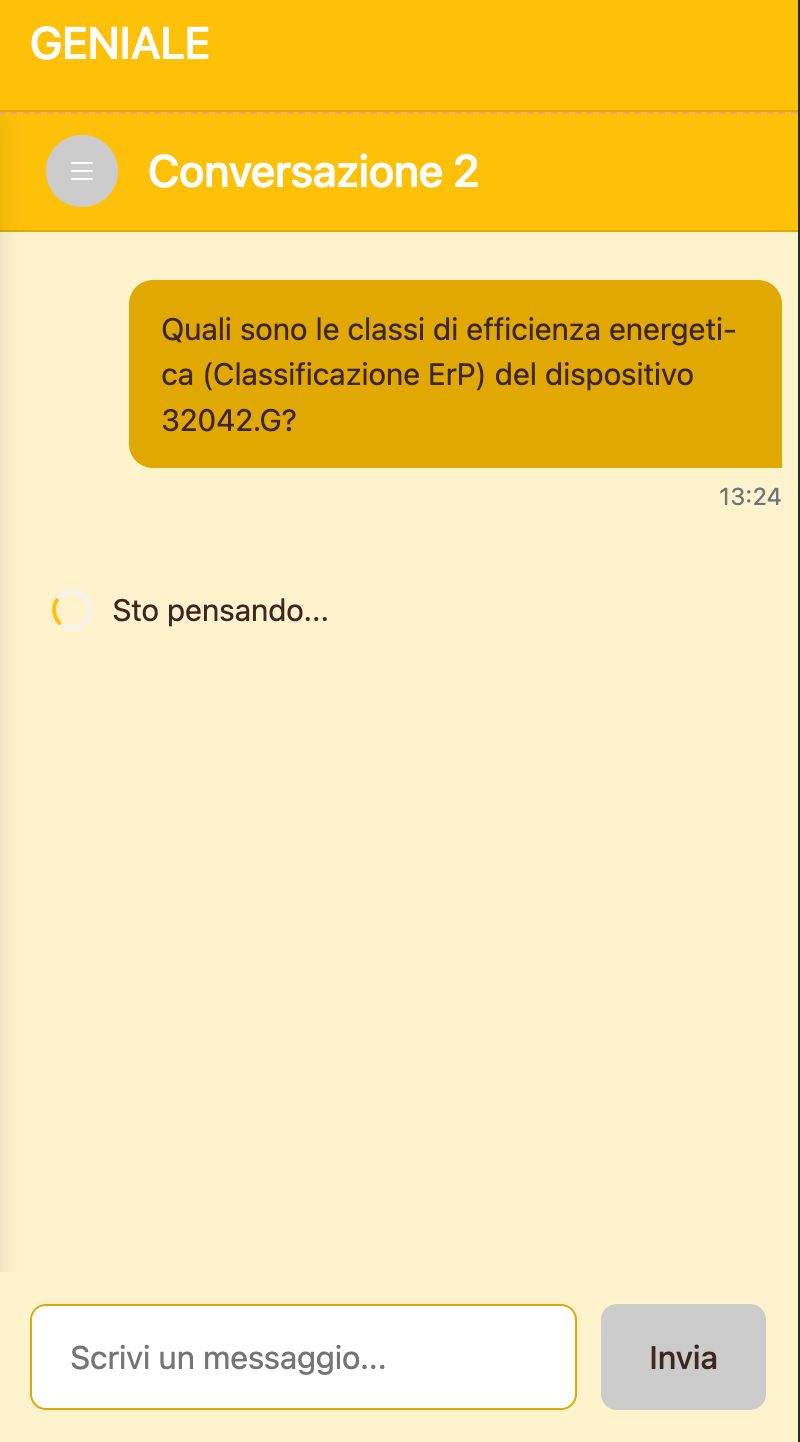
\includegraphics[width=0.5\textwidth]{contents/img/lock_mobile.jpg}
\caption{Limitazione delle interazioni durante l'attensa di una risposta}
\end{figure}
\end{document}
